\documentclass[table]{beamer}

\usepackage{pucv_jz}

\title{Inferencia}
\subtitle{Estadística Computacional}
\author[J.Z.O-2023]{Juan Zamora Osorio\\\url{juan.zamora@pucv.cl}}
\institute[PUCV]{Instituto de Estadística\\Pontificia Universidad Cat\'olica de Valpara\'iso}
\date{\today}

\begin{document}

\frame{\titlepage}

\begin{frame}
    \frametitle{Inferencia}
    \begin{block}{Hemos aprendido sobre...}
        \begin{itemize}
            \item Describir datos.
            \item Probabilidades.
            \item Variables aleatorias.
        \end{itemize}
    \end{block}
    \begin{block}{Objetivo}
        \begin{itemize}
            \item Contrastar datos reales con modelos basados en probabilidades.
        \end{itemize}
    \end{block}
    \begin{block}{¿Qué necesitamos?}
        \begin{itemize}
            \item Inferencia estadística.
            \item Contrastar hipótesis.
        \end{itemize}
    \end{block}
\end{frame}

\begin{frame}
    \frametitle{Recordar}
    \begin{block}{Probabilidades}
        \begin{itemize}
            \item ¿Dado un proceso que genera datos, cuáles son las propiedades que observaremos?
        \end{itemize}
    \end{block}
    \begin{center}
        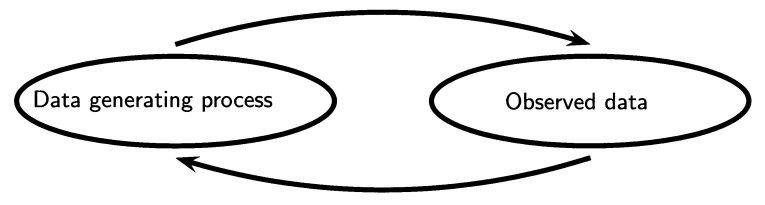
\includegraphics[height=0.3\textheight]{all2014_probabilidad_vs_inferencia}
    \end{center}
    \begin{block}{Inferencia estadística}
        \begin{itemize}
            \item ¿Dadas las observaciones, qué podemos decir sobre el proceso que genera los datos?
        \end{itemize}
    \end{block}
\end{frame}

\begin{frame}
    \frametitle{Recuerdo}
    \begin{block}{Media muestral}
        \begin{equation*}
            \bar{x} = \frac{x_{1} + x_{2} + \cdots + x_{n}}{n} = \frac{1}{n} \sum_{i = 1}^{n} x_{i} = \frac{\sum_{i = 1}^{n} x_{i}}{n}.
        \end{equation*}
        \begin{itemize}
            \item Busca estimar la \emph{media} de la población, denotada como $\mu$.
        \end{itemize}
    \end{block}
    \begin{block}{Ejemplo: temperaturas máximas durante enero}
        \begin{itemize}
            \item 22, 24, 21, 22, 25, 26, 25, 24, 23, 25, 25, 26, 27, 25, 26, 25, 26, 27, 27, 28, 29, 29, 29, 28, 30, 29, 30, 31, 30, 28, 29.
            \item $\bar{x} = \frac{22 + 24 + 21 + \cdots + 28 + 29}{31} = 26.48$ ºC.
        \end{itemize}
    \end{block}
\end{frame}

\begin{frame}
    \frametitle{Muestra}
    \begin{block}{Resultados obtenidos de experimentos aleatorios}
        \begin{itemize}
            \item Cantidad es finita.
            \item Generalmente se supone independencia.
            \item Generalmente se supone misma distribución en cada experimento.
        \end{itemize}
    \end{block}
    \begin{block}{Estadístico}
        \begin{itemize}
            \item Función calculada a partir de la muestra.
        \end{itemize}
    \end{block}
    \begin{block}{Ejemplo: $10$ lanzamientos de un dado}
        \begin{itemize}
            \item Cantidad de datos: $10$.
            \item Cada lanzamiento independiente del anterior.
            \item Cada lanzamiento posee la misma distribución: multinomial.
        \end{itemize}
    \end{block}
\end{frame}

\begin{frame}
    \frametitle{Muestra}
    \begin{block}{Ejemplo: $10$ tomas de temperatura a medio día en días distintos}
        \begin{itemize}
            \item Cantidad de datos: $10$.
            \item ¿Cada medición es independiente de la anterior?
            \item ¿Cada medición posee misma distribución?
        \end{itemize}
    \end{block}
    \begin{block}{Ejemplo: $10$ nombres de estudiantes del curso}
        \begin{itemize}
            \item Cantidad de datos: $10$.
            \item ¿Cada nombre es independiente del anterior?
            \item ¿Cada nombre posee la misma distribución?
        \end{itemize}
    \end{block}
    \begin{block}{}
        \begin{itemize}
            \item Queremos que la muestra sea representativa.
        \end{itemize}
    \end{block}
\end{frame}

\begin{frame}
    \frametitle{Técnicas de muestreo}
    \begin{block}{Sesgo}
        \begin{itemize}
            \item Una técnica es sesgada si el estadístico calculado con la muestra obtenida es mayor o menor, en promedio, que el parámetro estimado.
        \end{itemize}
    \end{block}
    \begin{block}{Sesgo de selección}
        \begin{itemize}
            \item La manera en que se construye la muestra introduce sesgo.
        \end{itemize}
    \end{block}
    \begin{block}{Sesgo de respuesta}
        \begin{itemize}
            \item La técnica para obtener la respuesta introduce sesgo.
        \end{itemize}
    \end{block}
\end{frame}

\begin{frame}
    \frametitle{Sesgo de selección}
    \begin{block}{Ejemplo -- tamaño}
        \begin{itemize}
            \item Los pacientes que pasan más días en un hospital son más propensos a ser elegidos para una muestra.
        \end{itemize}
    \end{block}
    \begin{block}{Ejemplo -- respuesta voluntaria}
        \begin{itemize}
            \item Las opiniones recolectadas por llamados a un programa de televisión sobre representan a quienes les importa el asunto y no representan a quienes no les interesa.
        \end{itemize}
    \end{block}
    \begin{block}{Ejemplo -- conveniencia}
        \begin{itemize}
            \item Selecciono a mis amigo/as como muestra para estudiar la opinión de la población.
        \end{itemize}
    \end{block}
\end{frame}

\begin{frame}
    \frametitle{Sesgo de selección}
    \begin{block}{Ejemplo -- juicio experto}
        \begin{itemize}
            \item Se intenta recolectar un grupo de personas con ciertas características: tantos hombres, tantas mujeres, tantos sobre 40, tantos empleados, etc. creyendo que se mejora representatividad, pero se agrega sesgo.
        \end{itemize}
    \end{block}
    \begin{block}{Ejemplo -- marco}
        \begin{itemize}
            \item Se selecciona a partir de una lista que debería corresponder a la población.
        \end{itemize}
    \end{block}
\end{frame}

\begin{frame}
    \frametitle{Sesgo de respuesta}
    \begin{block}{No hay respuesta}
        \begin{itemize}
            \item Alguien que se niega a participar en una encuesta podría ser diferente a los demás.
        \end{itemize}
    \end{block}
    \begin{block}{Respuesta incorrecta o error de medición}
        \begin{itemize}
            \item Mentira intencional.
            \item Memoria imprecisa.
            \item Medición imprecisa.
            \item Ejemplos:
                \begin{itemize}
                    \item Muchas personas no admiten ver un programa de televisión.
                    \item Pacientes que dicen que siguen indicaciones médicas.
                    \item ¿Cuánto tiempo pasan en el celular al día?
                \end{itemize}
        \end{itemize}
    \end{block}
\end{frame}

\begin{frame}
    \frametitle{Sesgo de respuesta}
       \begin{block}{Cuestionario}
        \begin{itemize}
            \item La respuesta depende de la pregunta, del tono de voz del entrevistador, el orden de las preguntas, etc.
        \end{itemize}
    \end{block}
\end{frame}

\begin{frame}
    \frametitle{Ejemplo: muestra de localización de daños en bombarderos}
    \begin{center}
        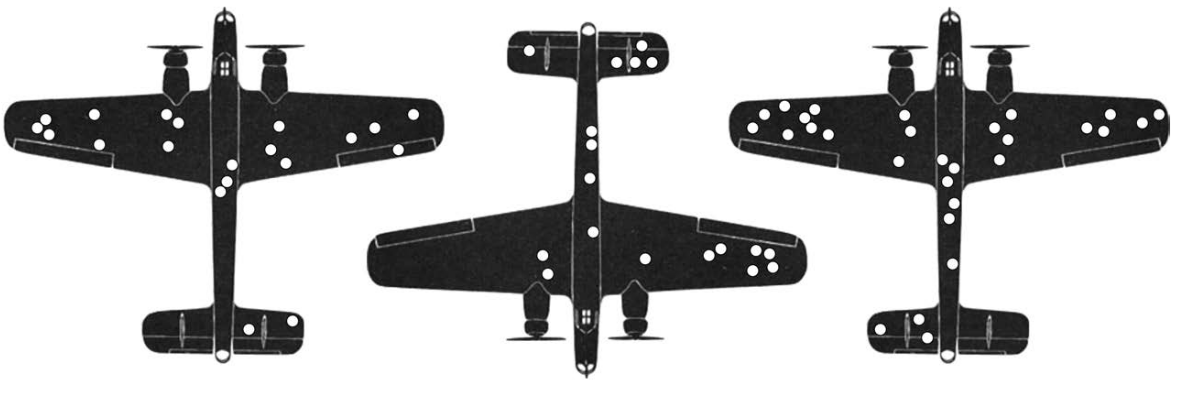
\includegraphics[width=\textwidth]{sesgo_aviones}
    \end{center}
\end{frame}

\begin{frame}
    \frametitle{Muestra aleatoria}
    \begin{block}{}
        \begin{itemize}
            \item No introduce sesgo.
        \end{itemize}
    \end{block}
    \begin{block}{Aleatoria simple}
        \begin{itemize}
            \item Todas las observaciones son igual de probables.
        \end{itemize}
        \begin{center}
            
\includegraphics[width=0.3\textwidth]{muestra_aleatoria_simple}
        \end{center}
    \end{block}
    \begin{block}{Aleatoria estratificada}
        \begin{itemize}
            \item Se divide la población en grupos que no se traslapan.
        \end{itemize}
        \begin{center}
            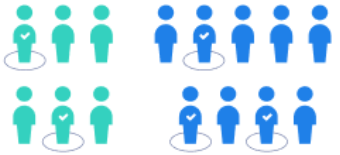
\includegraphics[width=0.3\textwidth]{muestra_aleatoria_estratificada}
        \end{center}
    \end{block}
\end{frame}

\begin{frame}
    \frametitle{Ejemplo: Plaza Pública CADEM}
    \begin{center}
        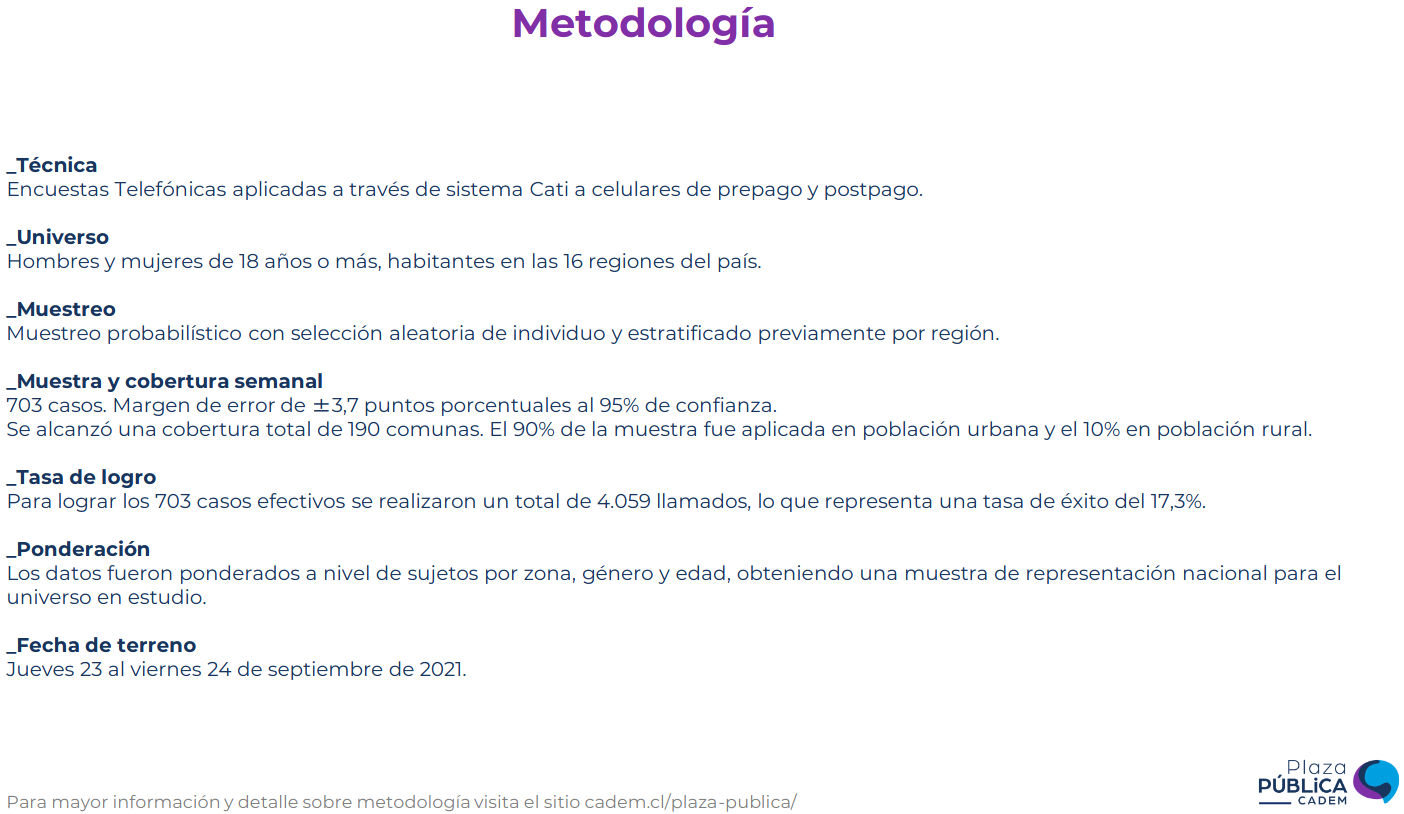
\includegraphics[width=\textwidth]{cadem}
    \end{center}
\end{frame}

\begin{frame}
    \frametitle{Muestra aleatoria}
    \begin{block}{Independientes e idénticamente distribuidos (\emph{iid})}
        \begin{itemize}
            \item Cantidad de datos finita.
            \item Cada dato es independiente del anterior.
            \item Cada dato posee misma distribución.
        \end{itemize}
    \end{block}
    \begin{block}{Inferencia}
        \begin{itemize}
            \item Como todos tienen misma distribución, podemos inferir sobre ella.
            \item Modelos estadísticos que suponen cantidad finita de parámetros se llaman \emph{paramétricos}.
            \item Ejemplo: $\normal{\mu}{\sigma^{2}}$ tiene solo dos parámetros.
            \item Un estadístico que busca estimar un parámetro de la población se llama \emph{estimador}.
        \end{itemize}
    \end{block}
\end{frame}

\begin{frame}
    \frametitle{Muestra aleatoria}
    \begin{block}{Independientes e idénticamente distribuidos (\emph{iid})}
        \begin{itemize}
            \item Cada dato puede modelarse como una variable aleatoria $X^{\parens{i}}$.
            \item Cada dato podría ser multivariado, $\Xvec^{\parens{i}} = \parens{X_{1}^{\parens{i}} , \ldots , X_{J}^{\parens{i}}}$.
            \item Matriz de datos:
                \begin{equation*}
                    \Xvec =
                    \begin{bmatrix}
                        \Xvec^{\parens{1} T} \\
                        \vdots \\
                        \Xvec^{\parens{i} T} \\
                        \vdots \\
                        \Xvec^{\parens{n} T}
                    \end{bmatrix}
                    =
                    \begin{bmatrix}
                        X_{1}^{\parens{1}} & \cdots & X_{j}^{\parens{1}} & \cdots & X_{J}^{\parens{1}} \\
                        \vdots & \ddots & \vdots & \ddots & \vdots \\
                        X_{1}^{\parens{i}} & \cdots & X_{j}^{\parens{i}} & \cdots & X_{J}^{\parens{i}} \\
                        \vdots & \ddots & \vdots & \ddots & \vdots \\
                        X_{1}^{\parens{n}} & \cdots & X_{j}^{\parens{n}} & \cdots & X_{J}^{\parens{n}}
                    \end{bmatrix}
                \end{equation*}
        \end{itemize}
    \end{block}
\end{frame}

\begin{frame}
    \frametitle{Media muestral}
    \begin{block}{Estadístico}
        \begin{itemize}
            \item Sea $\Xvec$ una muestra iid univariada.
            \item Sea $T_{n} = \sum_{i = 1}^{n} X^{\parens{i}}$, un estadístico.
            \item Sea $\bar{X}_{n} = \frac{1}{n} T_{n} = \frac{1}{n} \sum_{i = 1}^{n} X^{\parens{i}}$, un estadístico.
        \end{itemize}
    \end{block}
    \begin{block}{Propiedades}
        \begin{itemize}
            \item Si cada observación sigue una distribución con media $\mu$ y varianza $\sigma^{2}$:
            \item $\expected{\bar{X}_{n}} = \frac{1}{n} \sum_{i = 1}^{n} \expected{X^{\parens{i}}} = \frac{1}{n} n \mu = \mu$.
            \item $\variance{\bar{X}_{n}} = \frac{1}{n^{2}} \sum_{i = 1}^{n} \variance{X^{\parens{i}}} = \frac{1}{n^{2}} n \sigma^{2} = \frac{\sigma^{2}}{n}$.
        \end{itemize}
    \end{block}
    \begin{block}{}
        \begin{itemize}
            \item ¿Qué significa que $\bar{X}_{n}$ sea una variable aleatoria con media $\mu$ y varianza $\frac{\sigma^{2}}{n}$?
        \end{itemize}
    \end{block}
\end{frame}

\begin{frame}
    \frametitle{Sobre los estimadores}
    \begin{block}{Funciones de la muestra aleatoria}
        \begin{itemize}
            \item $\hat{\theta}_{n} = g \parens{X^{\parens{1}} , X^{\parens{2}} , \ldots , X^{\parens{n}}}$.
            \item Son estimadores \emph{puntuales}, nos entregan un valor para una muestra.
        \end{itemize}
    \end{block}
    \begin{block}{¡Son variables aleatorias!}
        \begin{itemize}
            \item Su valor depende del resultado de un experimento aleatorio.
        \end{itemize}
    \end{block}
    \begin{center}
        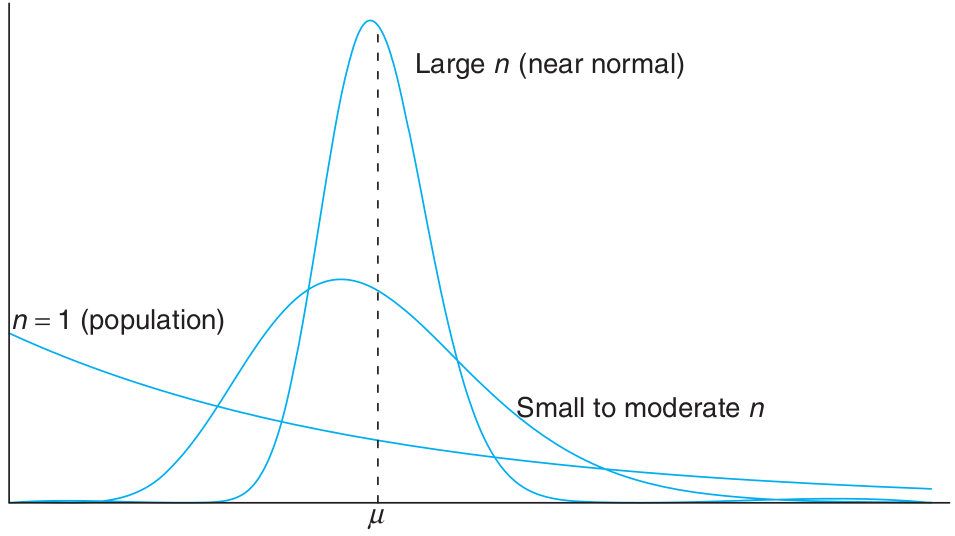
\includegraphics[height=0.35\textheight]{sampling_distribution}
    \end{center}
\end{frame}

\begin{frame}
    \frametitle{Media muestral}
    \begin{block}{Ejemplo: tragamonedas}
        \begin{itemize}
            \item Cada tirada tiene valor esperado $- \$ 1000$ y desviación estándar de $\$ 10000$.
            \item ¿Qué se espera en promedio luego de jugar...
                \begin{itemize}
                    \item $1$ vez?
                    \item $10$ veces?
                    \item $100$ veces?
                    \item $1000$ veces?
                \end{itemize}
        \end{itemize}
    \end{block}
    \begin{block}{Sabemos que}
        \begin{itemize}
            \item $\expected{X^{\parens{i}}} = - 1000$.
            \item $\variance{X^{\parens{i}}} = 10^{8}$.
            \item $\expected{\bar{X}_{n}} = - 1000$.
            \item $\variance{\bar{X}_{n}} = \frac{10^{8}}{n}$.
        \end{itemize}
    \end{block}
\end{frame}

\begin{frame}
    \frametitle{Media muestral -- simulación}
    \begin{block}{Ejemplo: tragamonedas}
        \begin{itemize}
            \item Suponiendo $X^{\parens{i}} \sim \uniform{- 3000}{1000}$.
            \item $1$ juego.
        \end{itemize}
    \end{block}
    \begin{center}
        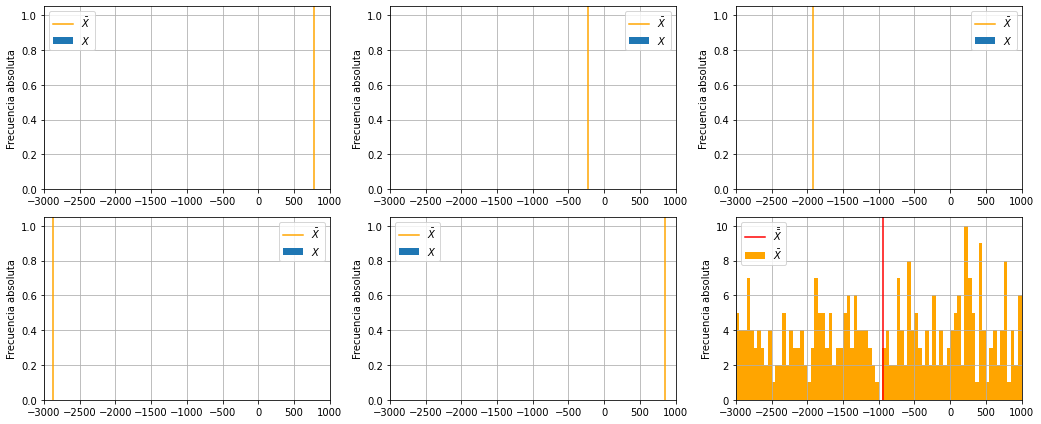
\includegraphics[width=\textwidth]{media_1}
    \end{center}
\end{frame}

\begin{frame}
    \frametitle{Media muestral -- simulación}
    \begin{block}{Ejemplo: tragamonedas}
        \begin{itemize}
            \item Suponiendo $X^{\parens{i}} \sim \uniform{- 3000}{1000}$.
            \item $10$ juegos.
        \end{itemize}
    \end{block}
    \begin{center}
        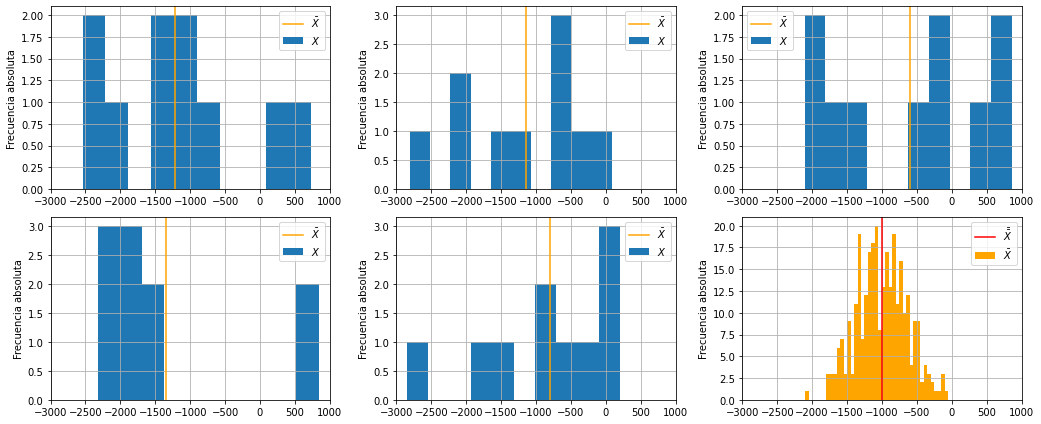
\includegraphics[width=\textwidth]{media_10}
    \end{center}
\end{frame}

\begin{frame}
    \frametitle{Media muestral -- simulación}
    \begin{block}{Ejemplo: tragamonedas}
        \begin{itemize}
            \item Suponiendo $X^{\parens{i}} \sim \uniform{- 3000}{1000}$.
            \item $100$ juegos.
        \end{itemize}
    \end{block}
    \begin{center}
        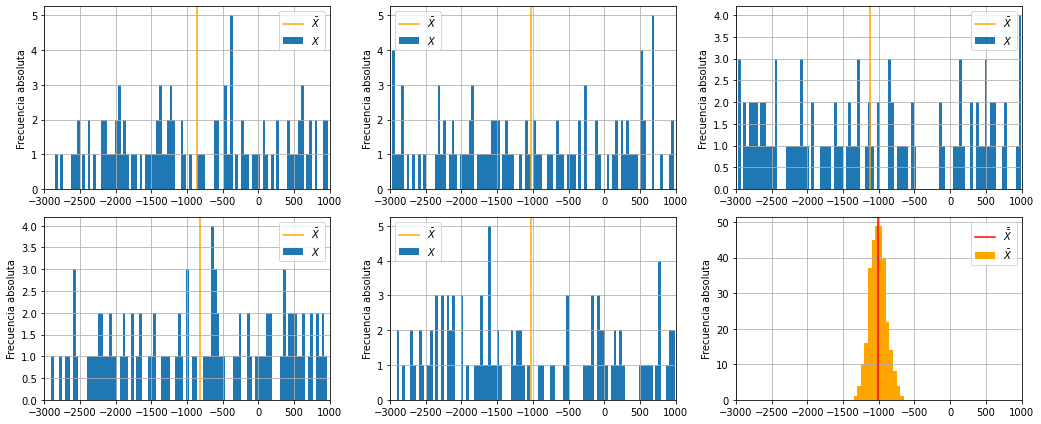
\includegraphics[width=\textwidth]{media_100}
    \end{center}
\end{frame}

\begin{frame}
    \frametitle{Media muestral -- simulación}
    \begin{block}{Ejemplo: tragamonedas}
        \begin{itemize}
            \item Suponiendo $X^{\parens{i}} \sim \uniform{- 3000}{1000}$.
            \item $1000$ juegos.
        \end{itemize}
    \end{block}
    \begin{center}
        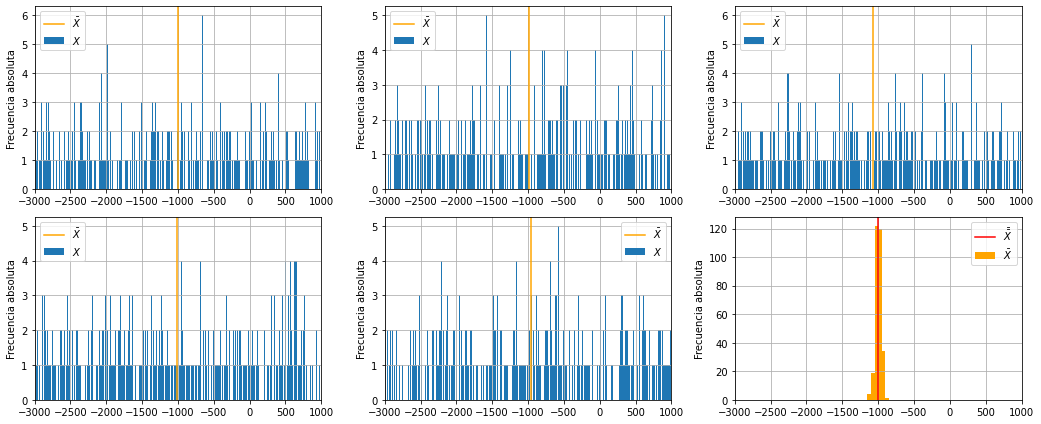
\includegraphics[width=\textwidth]{media_1000}
    \end{center}
\end{frame}

\begin{frame}
    \frametitle{Ley de los grandes números}
    \begin{block}{Media muestral}
        \begin{itemize}
            \item Sea $X$ una variable aleatoria con media $\mu$ y varianza $\sigma^{2}$.
            \item Sea $\bar{X}_{n} = \frac{1}{n} \sum_{i = 1}^{n} X^{\parens{i}}$ media de $n \in \naturals$ observaciones.
        \end{itemize}
    \end{block}
    \begin{block}{Teorema: Ley \emph{débil} de los grandes números}
        \begin{equation*}
            \lim_{n \rightarrow \infty} \prob{\vparens{\bar{X}_{n} - \mu} \geq \epsilon} = 0 .
        \end{equation*}
        \begin{itemize}
            \item Para todo $\epsilon > 0 \in \reals$ elegido se cumple.
            \item Para todo $\epsilon, \delta > 0 \in \reals$, existe $n \in \naturals$ tal que $\prob{\vparens{\bar{X}_{n} - \mu} \geq \epsilon} < \delta$.
        \end{itemize}
    \end{block}
\end{frame}

%%%%%%%%%%%%%%


\begin{frame}
    \frametitle{Nota: Tipos de convergencia}
    \begin{block}{En probabilidad (ley \emph{débil})}
        \begin{equation*}
            \lim_{n \rightarrow \infty} \prob{\vparens{\bar{X}_{n} - \mu} \geq \epsilon} = 0 .
        \end{equation*}
        \begin{itemize}
            \item Para todo $\epsilon, \delta > 0 \in \reals$, existe $n \in \naturals$ tal que $\prob{\vparens{\bar{X}_{n} - \mu} \geq \epsilon} < \delta$.
        \end{itemize}
        \begin{equation*}
            \bar{X}_{n} \overset{P}{\to} \mu .
        \end{equation*}
    \end{block}
\end{frame}

\begin{frame}
    \frametitle{Nota: Tipos de convergencia}
   \begin{block}{Casi segura o casi en todas partes (ley \emph{fuerte})}
        \begin{equation*}
            \prob{\lim_{n \rightarrow \infty} \bar{X}_{n} = \mu} = 1 .
        \end{equation*}
        \begin{itemize}
            \item Para toda secuencia infinita observada $\omega$, la media $\bar{X}_{n}$ converge a $\mu$, exceptuando, a lo más, un conjunto de probabilidad $0$.
        \end{itemize}
        \begin{equation*}
            \bar{X}_{n} \overset{\text{c.s.}}{\to} \mu .
        \end{equation*}
    \end{block}
\end{frame}


\begin{frame}
    \frametitle{Ley débil de los grandes números -- demostración}
    \begin{block}{Teorema: Ley \emph{débil} de los grandes números}
        \begin{equation*}
            \lim_{n \rightarrow \infty} \prob{\vparens{\bar{X}_{n} - \mu} \geq \epsilon} = 0 .
        \end{equation*}
        \begin{itemize}
            \item Para todo $\epsilon, \delta > 0 \in \reals$, existe $n \in \naturals$ tal que $\prob{\vparens{\bar{X}_{n} - \mu} \geq \epsilon} < \delta$.
        \end{itemize}
    \end{block}
    \begin{block}{Desigualdad de Chebyschev}
        \begin{itemize}
            \item Sea $k > 0 \in \reals$ y $X$ una variable aleatoria con media $\mu$ y varianza $\sigma^{2}$.
            \item Entonces:
        \end{itemize}
        \begin{equation*}
            \prob{\vparens{X - \mu} \geq k \sigma} \leq \frac{1}{k^{2}} .
        \end{equation*}
    \end{block}
\end{frame}

\begin{frame}
    \frametitle{Ley débil de los grandes números -- demostración}
    \begin{block}{Demostración desigualdad de Chebyschev}
        \begin{multline*}
            \prob{\vparens{X - \mu} \geq k \sigma}
            = \prob{X \leq \mu - k \sigma} + \prob{X \geq \mu + k \sigma}
            \\
            = \int_{- \infty}^{\mu - k \sigma} \ppdf{X}{x} dx
            + \int_{\mu + k \sigma}^{+ \infty} \ppdf{X}{x} dx
            \\
            \leq
            \int_{- \infty}^{\mu - k \sigma} \frac{\parens{x - \mu}^{2}}{k^{2}\sigma^{2}} \ppdf{X}{x} dx
            + \int_{\mu + k \sigma}^{+ \infty} \frac{\parens{x - \mu}^{2}}{k^{2}\sigma^{2}} \ppdf{X}{x} dx
            \\
            = \frac{1}{k^{2} \sigma^{2}} \parens{\int_{- \infty}^{\mu - k \sigma} \parens{x - \mu}^{2} \ppdf{X}{x} dx
            + \int_{\mu + k \sigma}^{+ \infty} \parens{x - \mu}^{2} \ppdf{X}{x} dx}
            \\
            %\leq \frac{1}{k^{2} \sigma^{2}} \parens{\int_{- \infty}^{\mu - k \sigma} \parens{x - \mu}^{2} \ppdf{X}{x} dx
            %+ \int_{\mu - k \sigma}^{\mu + k \sigma} \parens{x - \mu}^{2} \ppdf{X}{x} dx
            %+ \int_{\mu + k \sigma}^{+ \infty} \parens{x - \mu}^{2} \ppdf{X}{x} dx}
            %\\
            \leq \frac{1}{k^{2} \sigma^{2}}
            \int_{- \infty}^{+ \infty} \parens{x - \mu}^{2} \ppdf{X}{x} dx
            = \frac{1}{k^{2} \sigma^{2}} \sigma^{2}
            = \frac{1}{k^{2}}
            \\
            \Rightarrow
            \prob{\vparens{X - \mu} \geq k \sigma} \leq \frac{1}{k^{2}}
        \end{multline*}
    \end{block}
\end{frame}

\begin{frame}
    \frametitle{Ley débil de los grandes números -- demostración}
    \begin{block}{Teorema: Ley \emph{débil} de los grandes números}
        \begin{itemize}
            \item Para todo $\epsilon, \delta > 0 \in \reals$, existe $n \in \naturals$ tal que $\prob{\vparens{\bar{X}_{n} - \mu} \geq \epsilon} < \delta$:
                \begin{equation*}
                    \lim_{n \rightarrow \infty} \prob{\vparens{\bar{X}_{n} - \mu} \geq \epsilon} = 0 .
                \end{equation*}
        \end{itemize}
    \end{block}

\end{frame}

\begin{frame}
    \frametitle{Ley débil de los grandes números -- demostración}
   \begin{block}{Demostración}
        \begin{itemize}
            \item Sabemos que $\variance{\bar{X}_{n}} = \frac{\sigma^{2}}{n}$.
            \item Entonces, para todo $k > 0 \in \reals$:
                \begin{equation*}
                    \prob{\vparens{\bar{X}_{n} - \mu} \geq \frac{k \sigma}{\sqrt{n}}} \leq \frac{1}{k^{2}} .
                \end{equation*}
            \item Basta elegir $k = \frac{\epsilon \sqrt{n}}{\sigma}$ y se tiene:
                \begin{equation*}
                    \prob{\vparens{\bar{X}_{n} - \mu} \geq \epsilon} \leq \frac{\sigma^{2}}{\epsilon^{2} n} .
                \end{equation*}
            \item Finalmente, basta tomar $n > \frac{\sigma^{2}}{\epsilon^{2} \delta}$ y se tiene que
                 $\prob{\vparens{\bar{X}_{n} - \mu} \geq \epsilon} < \delta$.
        \end{itemize}
    \end{block}
\end{frame}


\begin{frame}
    \frametitle{Ley de los grandes números}
    \begin{block}{Ejemplo}
        \begin{itemize}
            \item Sea $X \sim \bernoulli{\frac{\pi}{4}}$.
            \item Sabemos que $\expected{X} = \mu = \frac{\pi}{4}$ y $\variance{X} = \sigma^{2} = \frac{\pi}{4} \parens{1 - \frac{\pi}{4}}$.
            \item Por ley de los grandes números, sabemos que $\bar{X}_{n}$ converge a $\mu = \frac{\pi}{4}$.
        \end{itemize}
    \end{block}
    \begin{block}{Cálculo de $\pi$}
        \begin{itemize}
            \item Obtenemos $n$ observaciones de $X$ y calculamos la media $\bar{X}_{n}$.
            \item Sabemos que $\bar{X}_{n} \to \frac{\pi}{4}$.
            \item Entonces, aproximamos $\pi \approx 4 \bar{X}_{n}$.
            \item ¿Y cómo obtenemos observaciones de $X$?
        \end{itemize}
    \end{block}
\end{frame}

\begin{frame}
    \frametitle{Ley de los grandes números}
    \begin{block}{Simulando $X \sim \bernoulli{\frac{\pi}{4}}$}
        \begin{itemize}
            \item Sean $X_{1} , X_{2} \sim \uniform{- \frac{1}{2}}{\frac{1}{2}}$.
            \item Sea $X = \begin{cases} 1 \text{ si } \parens{X_{1}, X_{2}} \text{ dentro de círculo radio } \frac{1}{2} \text{ y centro } \parens{0, 0} \\ 0 \text{ si no} \end{cases}$.
            \item Notar que el espacio muestral $\Omega = X_{1} \times X_{2}$ es un cuadrado de lado $1$.
            \item El área que corresponde a $X = 1$ es el área del cículo de radio $\frac{1}{2}$.
            \item $\prob{X = 1} = \frac{\pi}{4}$ y $\prob{X = 0} = 1 - \frac{\pi}{4}$. Es decir, $X \sim \bernoulli{\frac{\pi}{4}}$.
        \end{itemize}
    \end{block}
%    \begin{center}
%        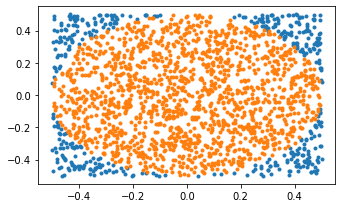
\includegraphics[width=0.45\textwidth]{montecarlo_pi}
%    \end{center}

\begin{tikzpicture}[remember picture, overlay]
\node[yshift=1.3cm, xshift=2cm] at (current page.south) 
{
    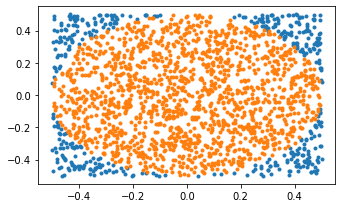
\includegraphics[width=0.35\textwidth]{montecarlo_pi}
};
\end{tikzpicture}  

\end{frame}

\begin{frame}
    \frametitle{Aproximando $\pi$}
    \begin{center}
        \setlength{\tabcolsep}{0pt}
        \begin{tabular}{cccc}
            $n = 100$ & $n = 1000$ & $n =10000$ & $n = 100000$ \\
            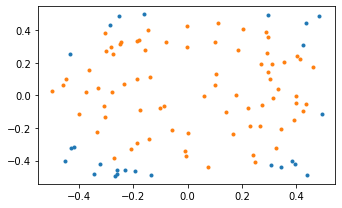
\includegraphics[width=0.25\textwidth]{montecarlo_pi_1_1}
            & 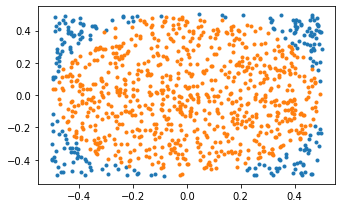
\includegraphics[width=0.25\textwidth]{montecarlo_pi_1_2}
            & 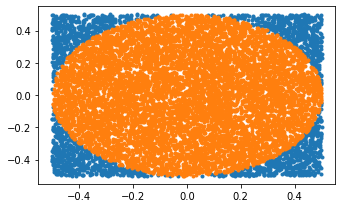
\includegraphics[width=0.25\textwidth]{montecarlo_pi_1_3}
            & 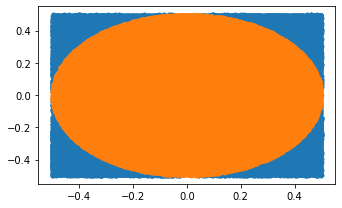
\includegraphics[width=0.25\textwidth]{montecarlo_pi_1_4}
            \\
            $\pi \approx 3.00$
            & $\pi \approx 3.088$
            & $\pi \approx 3.1616$
            & $\pi \approx 3.13976$
            \\
            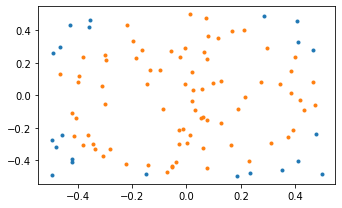
\includegraphics[width=0.25\textwidth]{montecarlo_pi_2_1}
            & 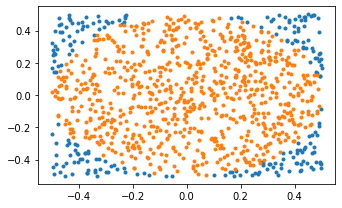
\includegraphics[width=0.25\textwidth]{montecarlo_pi_2_2}
            & 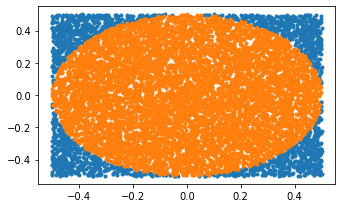
\includegraphics[width=0.25\textwidth]{montecarlo_pi_2_3}
            & 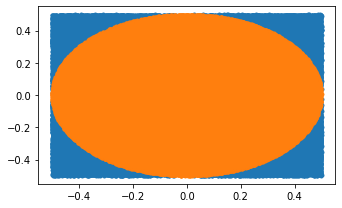
\includegraphics[width=0.25\textwidth]{montecarlo_pi_2_4}
            \\
            $\pi \approx 3.12$
            & $\pi \approx 3.104$
            & $\pi \approx 3.1652$
            & $\pi \approx 3.14968$
            \\
            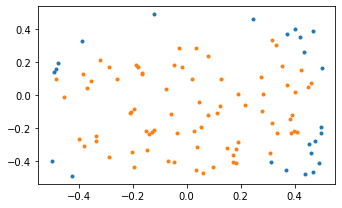
\includegraphics[width=0.25\textwidth]{montecarlo_pi_3_1}
            & 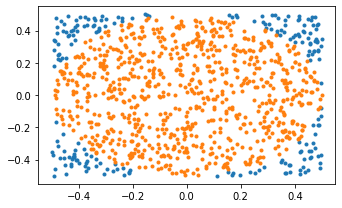
\includegraphics[width=0.25\textwidth]{montecarlo_pi_3_2}
            & 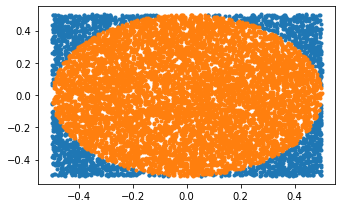
\includegraphics[width=0.25\textwidth]{montecarlo_pi_3_3}
            & 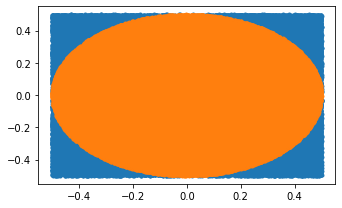
\includegraphics[width=0.25\textwidth]{montecarlo_pi_3_4}
            \\
            $\pi \approx 3.04$
            & $\pi \approx 3.164$
            & $\pi \approx 3.1496$
            & $\pi \approx 3.14356$
        \end{tabular}
    \end{center}
\end{frame}

\begin{frame}
    \frametitle{Aproximando $\pi$}
    \begin{center}
        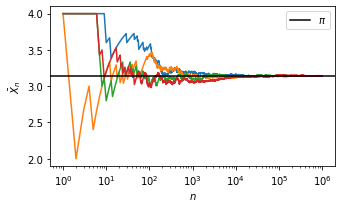
\includegraphics[width=0.49\textwidth]{montecarlo_pi_tray1}
        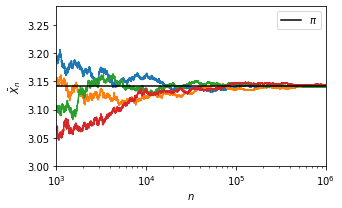
\includegraphics[width=0.49\textwidth]{montecarlo_pi_tray2}
    \end{center}
    \begin{block}{}
        \begin{itemize}
            \item Esta metodología se llama aproximación de Monte Carlo.
        \end{itemize}
    \end{block}
\end{frame}

\begin{frame}
    \frametitle{Teorema del límite central}
    \begin{block}{Media muestral}
        \begin{itemize}
            \item Sea $X$ una variable aleatoria con media $\mu$ y varianza $\sigma^{2}$.
            \item Sea $T_{n} = \sum_{i = 1}^{n} X^{\parens{i}}$, suma de $n \in \naturals$ observaciones.
            \item Sea $\bar{X}_{n} = \frac{1}{n} T_{n} = \frac{1}{n} \sum_{i = 1}^{n} X^{\parens{i}}$ media de $n \in \naturals$ observaciones.
        \end{itemize}
    \end{block}
    \begin{block}{Teorema}
        \begin{itemize}
            \item La variable aleatoria $Z_{n}$ siguiente converge a una distribución normal estándar $\normal{0}{1}$:
                \begin{equation*}
                    Z_{n} = \frac{T_{n} - n \mu}{\sigma \sqrt{n}}
                    = \frac{\bar{X}_{n} - \mu}{\frac{\sigma}{\sqrt{n}}}
                \end{equation*}
            \item Equivalentemente, $\bar{X}_{n} \sim \normal{\mu}{\frac{\sigma^{2}}{n}}$.
        \end{itemize}
    \end{block}
\end{frame}

\begin{frame}
    \frametitle{Media muestral -- simulación}
    \begin{block}{Ejemplo: tragamonedas}
        \begin{itemize}
            \item Suponiendo $Y^{\parens{i}} \sim \betadist{0.5}{1.5}$ y $X^{\parens{i}} = 4000 Y^{\parens{i}} - 3000$.
            \item $1$ juego.
        \end{itemize}
    \end{block}
    \begin{center}
        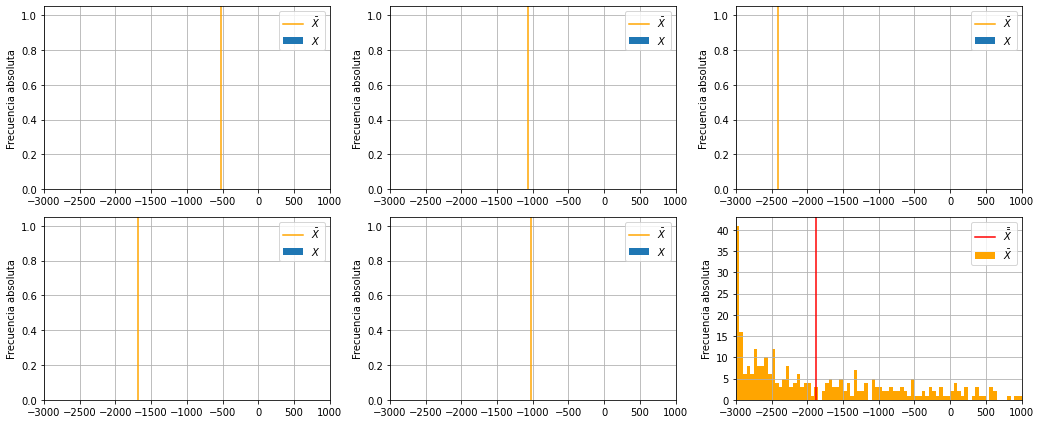
\includegraphics[width=\textwidth]{media_beta1}
    \end{center}
\end{frame}

\begin{frame}
    \frametitle{Media muestral -- simulación}
    \begin{block}{Ejemplo: tragamonedas}
        \begin{itemize}
            \item Suponiendo $Y^{\parens{i}} \sim \betadist{0.5}{1.5}$ y $X^{\parens{i}} = 4000 Y^{\parens{i}} - 3000$.
            \item $10$ juegos.
        \end{itemize}
    \end{block}
    \begin{center}
        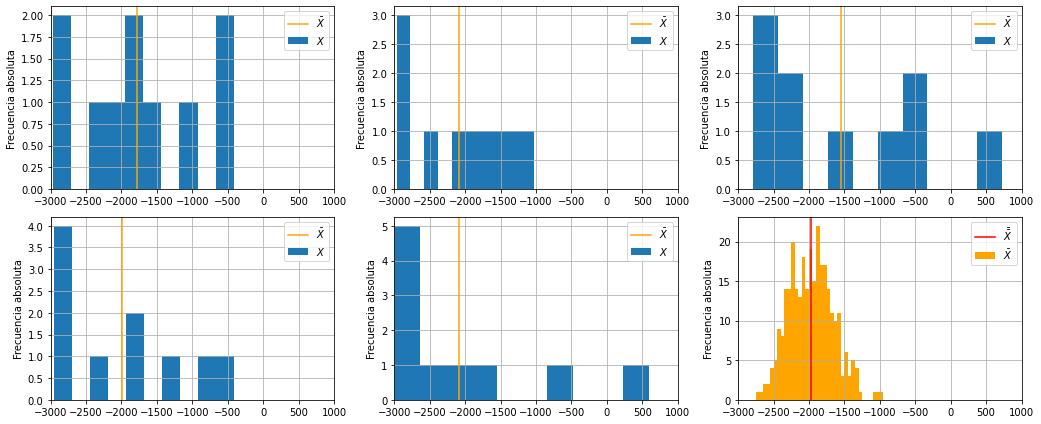
\includegraphics[width=\textwidth]{media_beta10}
    \end{center}
\end{frame}

\begin{frame}
    \frametitle{Media muestral -- simulación}
    \begin{block}{Ejemplo: tragamonedas}
        \begin{itemize}
            \item Suponiendo $Y^{\parens{i}} \sim \betadist{0.5}{1.5}$ y $X^{\parens{i}} = 4000 Y^{\parens{i}} - 3000$.
            \item $100$ juegos.
        \end{itemize}
    \end{block}
    \begin{center}
        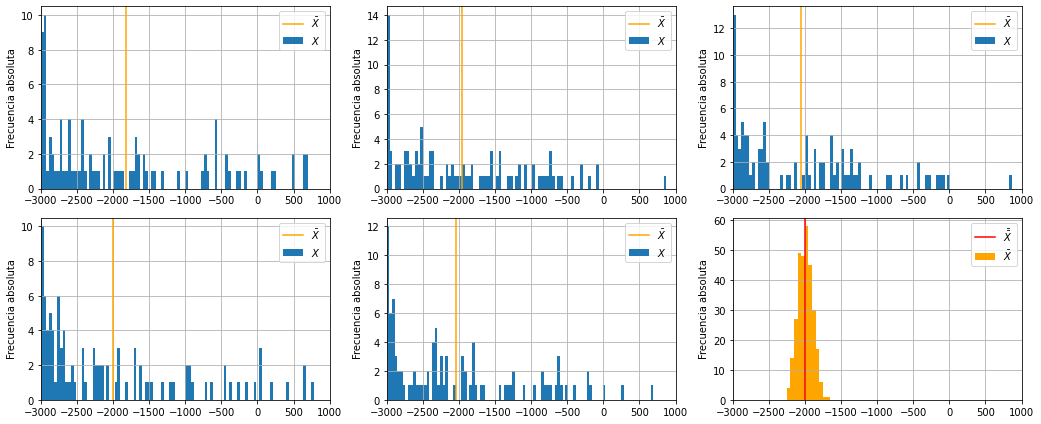
\includegraphics[width=\textwidth]{media_beta100}
    \end{center}
\end{frame}

\begin{frame}
    \frametitle{Media muestral -- simulación}
    \begin{block}{Ejemplo: tragamonedas}
        \begin{itemize}
            \item Suponiendo $Y^{\parens{i}} \sim \betadist{0.5}{1.5}$ y $X^{\parens{i}} = 4000 Y^{\parens{i}} - 3000$.
            \item $1000$ juegos.
        \end{itemize}
    \end{block}
    \begin{center}
        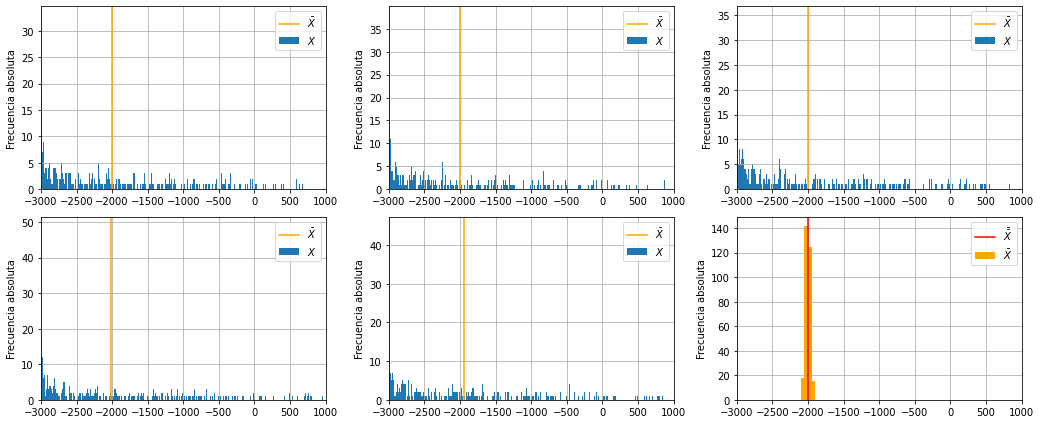
\includegraphics[width=\textwidth]{media_beta1000}
    \end{center}
\end{frame}

\begin{frame}
    \frametitle{Ejemplo: aproximación de Monte Carlo de $\pi$}
    \begin{block}{Supuesto}
        \begin{itemize}
            \item $X \sim \bernoulli{\frac{\pi}{4}}$.
            \item $\expected{X} = \mu = \frac{\pi}{4}$.
            \item $\variance{X} = \sigma^{2} = \frac{\pi}{4} \parens{1 - \frac{\pi}{4}}$.
        \end{itemize}
    \end{block}
    \begin{center}
        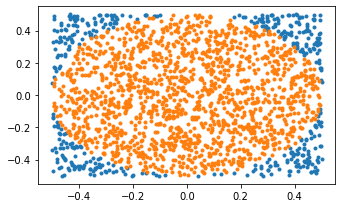
\includegraphics[width=0.45\textwidth]{montecarlo_pi}
    \end{center}
    \begin{block}{Teorema del límite central}
        \begin{itemize}
            \item $\bar{X}_{n} \sim \normal{\frac{\pi}{4}}{\frac{\frac{\pi}{4} \parens{1 - \frac{\pi}{4}}}{n}}$
        \end{itemize}
    \end{block}
\end{frame}

\begin{frame}
    \frametitle{Ejemplo: aproximación de Monte Carlo de $\pi$}
    \begin{block}{Teorema del límite central}
        \begin{itemize}
            \item $\bar{X}_{n} \sim \normal{\frac{\pi}{4}}{\frac{\frac{\pi}{4} \parens{1 - \frac{\pi}{4}}}{n}}$.
                Si $Y_{n} = 4 \bar{X}_{n}$, entonces $Y_{n} \sim \normal{\pi}{\frac{\pi \parens{4 - \pi}}{n}}$.
        \end{itemize}
    \end{block}
    \begin{center}
        \setlength{\tabcolsep}{0pt}
        \begin{tabular}{ccccc}
            $n$ & $100$ & $1000$ & $10000$ & $100000$ \\
            \hline
            Secuencia $1$ & $3.00$ & $3.088$ & $3.1616$ & $3.13976$ \\
            Secuencia $2$ & $3.12$ & $3.104$ & $3.1652$ & $3.14968$ \\
            Secuencia $3$ & $3.04$ & $3.164$ & $3.1496$ & $3.14356$ \\
            \hline
            $\expected{Y_{n}}$ & $3.14$ & $3.142$ & $3.1416$ & $3.14159$ \\
            % $\variance{Y_{n}}$ & $0.03$ & $0.003$ & $0.0003$ & $0.00003$ \\
            $\sqrt{\variance{Y_{n}}}$ & $0.16$ & $0.052$ & $0.0164$ & $0.00519$ \\
            & 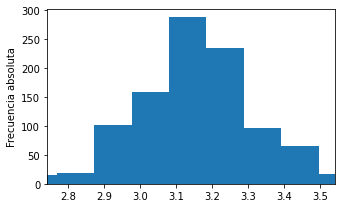
\includegraphics[width=0.21\textwidth]{media_tcl1} &
            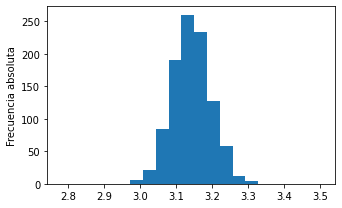
\includegraphics[width=0.21\textwidth]{media_tcl2} &
            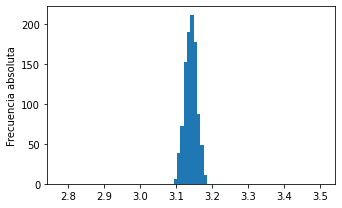
\includegraphics[width=0.21\textwidth]{media_tcl3} &
            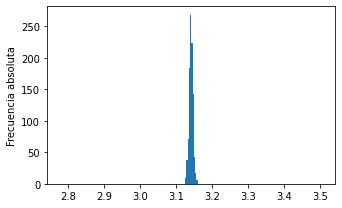
\includegraphics[width=0.21\textwidth]{media_tcl4}
        \end{tabular}
    \end{center}
\end{frame}

\begin{frame}
    \frametitle{Algunas aproximaciones}
    \begin{block}{Media}
        \begin{equation*}
            \bar{X}_{n} = \frac{1}{n} \sum_{i = 1}^{n} X^{\parens{i}} \to \expected{X} .
        \end{equation*}
    \end{block}
    \begin{block}{Varianza (con media conocida)}
        \begin{equation*}
            S^{2}_{n} = \frac{1}{n} \sum_{i = 1}^{n} \parens{X^{\parens{i}} - \expected{X}}^{2} \to \variance{X} = \expected{\parens{X - \expected{X}}^{2}} .
        \end{equation*}
    \end{block}
    \begin{block}{Función de distribución acumulada}
        \begin{equation*}
            \frac{1}{n} \vparens{\bparens{X^{\parens{i}} \text{ tal que } X^{\parens{i}} \leq c}} \to \pFF{X}{c} = \expected{\indicator{\parens{- \infty , c}}{X}} .
        \end{equation*}
    \end{block}
    %\begin{block}{Mediana}
    %    \begin{equation*}
    %        \tilde{X}_{n} = \text{mediana} \bparens{X^{\parens{1}}, \ldots , X^{\parens{i}} , \ldots , X^{\parens{n}}} \to \text{mediana} \parens{X} .
    %    \end{equation*}
    %\end{block}
\end{frame}

\begin{frame}
    \frametitle{Ejemplo}
    \begin{block}{Errores en un programa computacional}
        \begin{itemize}
            \item Sea $X$ variable aleatoria asociada a cantidad de errores por semana.
            \item Supongamos $X$ sigue una distribución de Poisson $\poisson{\lambda = 5}$.
            \item Hay $125$ programas independientes corriendo.
            \item ¿Probabilidad de que cantidad de errores promedio sea menor a $5.5$?
        \end{itemize}
    \end{block}
\end{frame}

\begin{frame}
    \frametitle{Ejemplo}
    \begin{block}{Errores en un programa computacional}
        \begin{itemize}
            \item Sea $X$ variable aleatoria asociada a cantidad de errores por semana.
            \item Supongamos $X$ sigue una distribución de Poisson $\poisson{\lambda = 5}$.
            \item Hay $125$ programas independientes corriendo.
            \item ¿Probabilidad de que cantidad de errores promedio sea menor a $5.5$?
        \end{itemize}
    \end{block}
    \begin{block}{Desarrollo}
        \begin{itemize}
            \item $\expected{X} = \mu = 5$.
            \item $\variance{X} = \sigma^{2} = 5$.
            \item Sabemos que $\bar{X}_{125}$ se parece a $\normal{\mu}{\frac{\sigma^{2}}{125}} = \normal{5}{\frac{1}{25}}$.
                \begin{equation*}
                    \prob{\bar{X}_{125} < 5.5} = \pFF{\bar{X}_{125}}{5.5} = \Phi \parens{\frac{5.5 - 5}{\sqrt{\frac{1}{25}}}}
                    %= \Phi \parens{\frac{5}{2}}
                    = \Phi \parens{2.5} \approx 0.9938
                    .
                \end{equation*}
        \end{itemize}
    \end{block}
\end{frame}

\begin{frame}
    \frametitle{Intervalos de confianza}
    \begin{block}{Errores en un programa computacional}
        \begin{itemize}
            \item Sea $X$ variable aleatoria asociada a cantidad de errores por semana.
            \item Supongamos $X$ sigue una distribución con media desconocida $\mu$ y varianza $\sigma^{2} = 5$.
            \item Hay $125$ programas independientes corriendo una semana.
            \item Medimos la cantidad de errores promedio, obteniendo $\bar{x}_{125} = 6$.
            \item $\bar{x}_{125} = 6$ es una estimación puntual de $\mu$.
            \item ¿Entre qué valores está $\mu$, con un $89\%$ de probabilidad?
        \end{itemize}
    \end{block}
    \begin{center}
        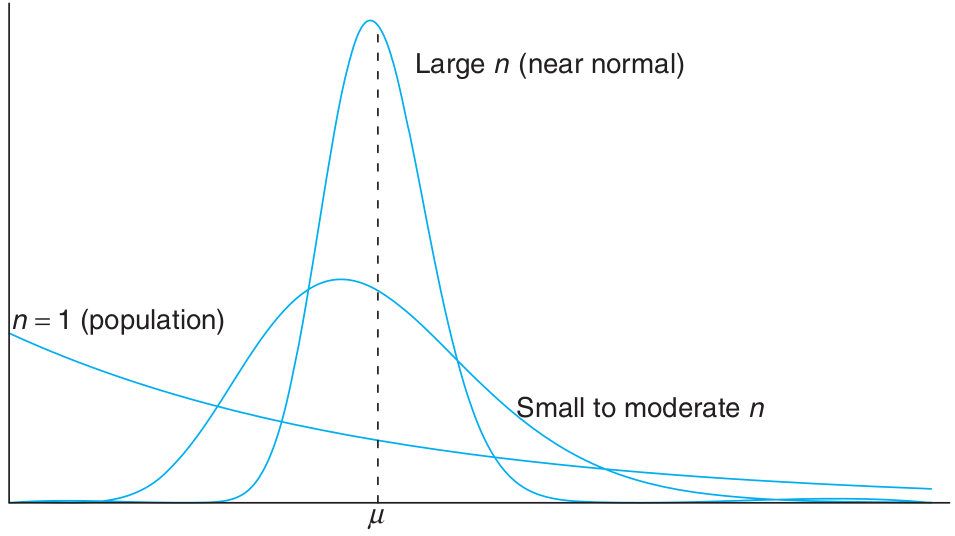
\includegraphics[height=0.35\textheight]{sampling_distribution}
    \end{center}
\end{frame}

\begin{frame}
    \frametitle{Intervalos de confianza}
    \begin{block}{Errores en un programa computacional}
        \begin{itemize}
            \item $\bar{x}_{125} = 6$ es una estimación puntual de $\mu$.
            \item ¿Entre qué valores está $\mu$, con un $89\%$ de probabilidad?
        \end{itemize}
    \end{block}
    \begin{block}{Desarrollo}
        \begin{itemize}
            \item Sabemos que $\bar{X}_{125}$ se parece a $\normal{\mu}{\frac{\sigma^{2}}{125}} = \normal{\mu}{\frac{1}{25}}$.
            \item Podemos escribir $\bar{X}_{125} \approx \frac{1}{5} Z + \mu$, con $Z \sim \normal{0}{1}$.
            \item Buscamos el intervalo centrado en $0$ para $Z$:
                \begin{equation*}
                    \prob{-1.598 \leq Z < 1.598} \approx 0.89 .
                \end{equation*}
            \item Resolvemos para $\mu$:
                \begin{multline*}
                    \prob{-1.598 \leq 5 \parens{\bar{X}_{125} - \mu} < 1.598} \approx 0.89
                    \\
                    \Rightarrow - 6.32 \leq - \mu < - 5.68
                    \Rightarrow \mu \in \left ( 5.68 , 6.32 \right ]
                    .
                \end{multline*}
        \end{itemize}
    \end{block}
\end{frame}

\begin{frame}
    \frametitle{Intervalos de confianza}
    \begin{block}{En general}
        \begin{itemize}
            \item Dado un $\alpha \in \sparens{0, 1}$.
            \item Buscamos un intervalo con un nivel dado de \emph{confianza} $1 - \alpha$.
            \item En este curso vamos a suponer intervalos centrados.
        \end{itemize}
    \end{block}
    \begin{center}
        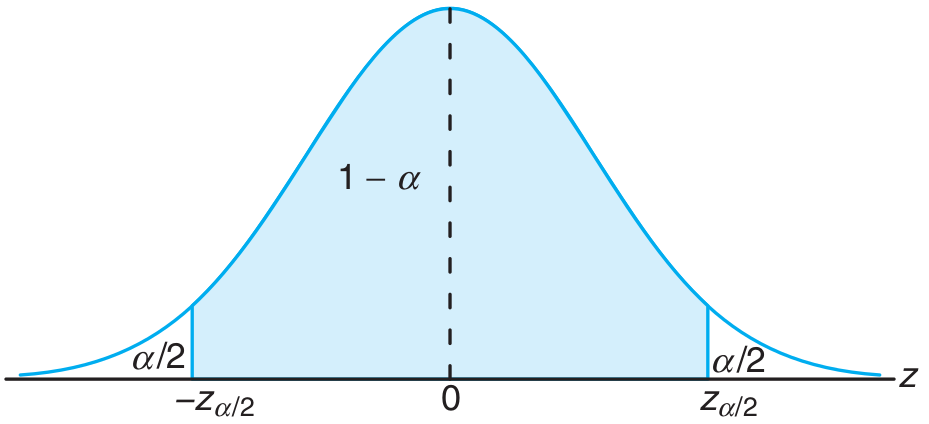
\includegraphics[height=0.5\textheight]{intervalo_1}
    \end{center}
\end{frame}

\begin{frame}
    \frametitle{Intervalos de confianza}
    \begin{block}{Si conocemos varianza $\sigma^{2}$ y queremos estimar $\mu$}
        \begin{itemize}
            \item Sabemos que $\bar{X}_{n}$ se parece a $\normal{\mu}{\frac{\sigma^{2}}{n}}$.
            \item Podemos escribir $\bar{X}_{n} \approx \frac{\sigma}{\sqrt{n}} Z + \mu$, con $Z \sim \normal{0}{1}$.
            \item Buscamos intervalo centrado para $Z$:
                $\prob{- z_{\frac{\alpha}{2}} \leq Z < z_{\frac{\alpha}{2}}} = 1 - \alpha$.
            \item Resolvemos para $\mu$:
                \begin{multline*}
                    \prob{- z_{\frac{\alpha}{2}} \leq \sqrt{n} \frac{\bar{X}_{n} - \mu}{\sigma} < z_{\frac{\alpha}{2}}}
                    = 1 - \alpha
                    \\
                    \Rightarrow
                    \bar{X}_{n} - \frac{\sigma}{\sqrt{n}} z_{\frac{\alpha}{2}} < \mu \leq \bar{X}_{n} + \frac{\sigma}{\sqrt{n}} z_{\frac{\alpha}{2}}
                    .
                \end{multline*}
        \end{itemize}
    \end{block}
    \begin{center}
        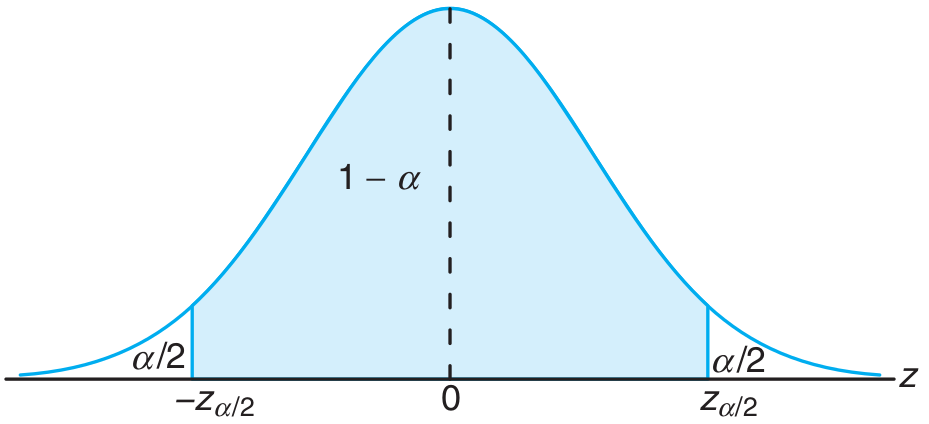
\includegraphics[height=0.24\textheight]{intervalo_1}
    \end{center}
\end{frame}

\begin{frame}
    \frametitle{Intervalos de confianza}
    \begin{block}{Límites del intervalo}
        \begin{itemize}
            \item Notar que $\bar{X}_{n} - \frac{\sigma}{\sqrt{n}} z_{\frac{\alpha}{2}}$ y $\bar{X}_{n} + \frac{\sigma}{\sqrt{n}} z_{\frac{\alpha}{2}}$ son variables aleatorias...
        \end{itemize}
    \end{block}
    \begin{center}
        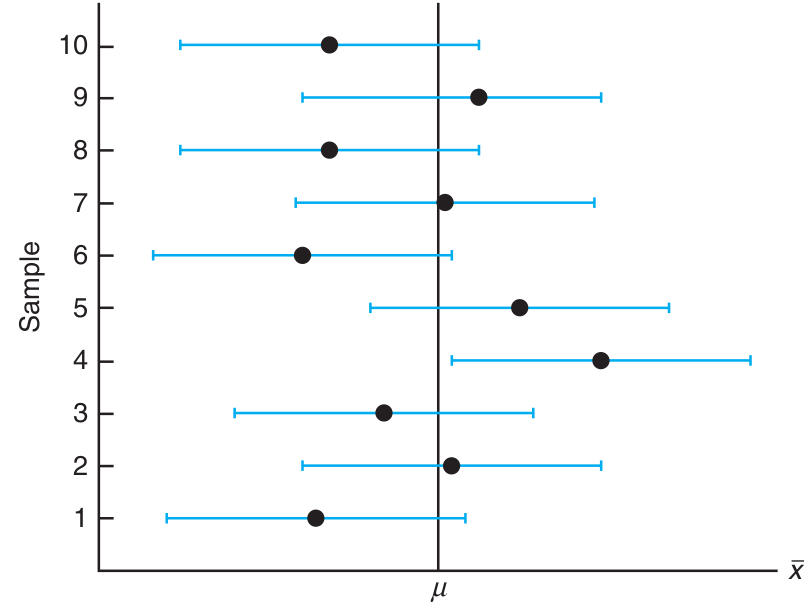
\includegraphics[height=0.48\textheight]{intervalo_ejemplos}
    \end{center}
    \begin{block}{Nota: \emph{Bootstrap}}
        \begin{itemize}
            \item Obtener intervalos de confianza usando distintas muestras generadas basadas la muestra original, con repetición.
        \end{itemize}
    \end{block}
\end{frame}

\begin{frame}
    \frametitle{Intervalos de confianza}
    \begin{block}{Frecuentista}
        \begin{itemize}
            \item En este caso $\mu$ tiene un valor fijo.
            \item La distribución es de $\bar{X}_{n}$ y los límites del intervalo.
        \end{itemize}
    \end{block}
    \begin{block}{Interpretación}
        \begin{itemize}
            \item Si se usa $\bar{X}_{n}$ para estimar $\mu$, se tiene confianza de $1 - \alpha$ de que el error no excede $\frac{\sigma}{\sqrt{n}} z_{\frac{\alpha}{2}}$.
        \end{itemize}
    \end{block}
    \begin{center}
        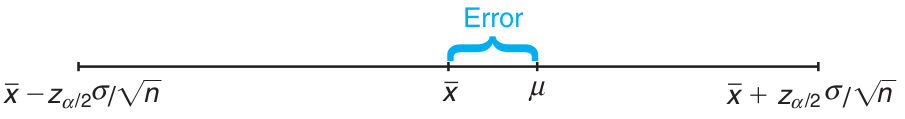
\includegraphics[width=\textwidth]{intervalo_error}
    \end{center}
    \begin{block}{Interpretación}
        \begin{itemize}
            \item Si se usa $\bar{X}_{n}$ para estimar $\mu$, se tiene confianza de $1 - \alpha$ de que el error no excede $e$ cuando la muestra es de tamaño $n = \parens{\frac{\sigma}{e} z_{\frac{\alpha}{2}}}^{2}$.
        \end{itemize}
    \end{block}
\end{frame}

\begin{frame}
    \frametitle{Intervalos de confianza}
    \begin{block}{Si no conocemos varianza $\sigma^{2}$ y queremos estimar $\mu$}
        \begin{itemize}
            \item Supongamos que $X^{\parens{i}}$ tiene distribución normal $\normal{\mu}{\sigma^{2}}$.
            \item Podemos estimar $\sigma^{2}$ con el estadístico varianza muestral
                \begin{equation*}
                    S^{2}_{n} = \frac{1}{n - 1} \sum_{i = 1}^{n} \parens{X^{\parens{i}} - \bar{X}_{n}}^{2} .
                \end{equation*}
        \end{itemize}
    \end{block}
    \begin{block}{Distribución de la media y varianza muestrales}
        \begin{itemize}
            \item Sabemos que $\bar{X}_{n} \sim \normal{\mu}{\frac{\sigma^{2}}{n}}$.
            \item Sabemos que $Z = \frac{\sqrt{n} \parens{\bar{X}_{n} - \mu}}{\sigma}$ es normal estándar, $Z \sim \normal{0}{1}$.
            \item $V =  \frac{\parens{n - 1} S^{2}_{n}}{\sigma^{2}}$ tiene distribución ji al cuadrado con $n - 1$ grados de libertad, $V \sim \chidist{n - 1}$:
                \begin{equation*}
                    \ppdf{V}{v} = \frac{1}{2^{\frac{n - 1}{2}} \gammafunc{\frac{n - 1}{2}}} v^{\frac{n - 1}{2} - 1} e^{- \frac{v}{2}} ,
                    \text{ con } v \in \left [ 0 , + \infty \right ) .
                \end{equation*}
        \end{itemize}
    \end{block}
\end{frame}

\begin{frame}
    \frametitle{Intervalos de confianza}
    \begin{block}{Distribución de la media y varianza muestrales}
        \begin{itemize}
            \item Sabemos que $\bar{X}_{n} \sim \normal{\mu}{\frac{\sigma^{2}}{n}}$.
            \item Sabemos que $Z = \frac{\sqrt{n} \parens{\bar{X}_{n} - \mu}}{\sigma}$ es normal estándar, $Z \sim \normal{0}{1}$.
            \item $V =  \frac{\parens{n - 1} S^{2}_{n}}{\sigma^{2}}$ tiene distribución ji al cuadrado con $n - 1$ grados de libertad, $V \sim \chidist{n - 1}$:
                \begin{equation*}
                    \ppdf{V}{v} = \frac{1}{2^{\frac{n - 1}{2}} \gammafunc{\frac{n - 1}{2}}} v^{\frac{n - 1}{2} - 1} e^{- \frac{v}{2}} ,
                    \text{ con } v \in \left [ 0 , + \infty \right ) .
                \end{equation*}
        \end{itemize}
    \end{block}
    \begin{block}{Teorema}
        \begin{itemize}
            \item La variable aleatoria $T = \frac{Z}{\sqrt{\frac{V}{n - 1}}}$ es distribución $t$ de Student con $n - 1$ grados de libertad:
                \begin{equation*}
                    \ppdf{T}{t} = \frac{\gammafunc{\frac{n}{2}}}{\gammafunc{\frac{n - 1}{2}} \sqrt{\pi \parens{n - 1}}} \parens{1 + \frac{t^{2}}{n - 1}}^{- \frac{n}{2}} .
                \end{equation*}
        \end{itemize}
    \end{block}
\end{frame}

\begin{frame}
    \frametitle{Intervalos de confianza}
    \begin{block}{Distribución de la media y varianza muestrales}
        \begin{itemize}
            \item Sabemos que $Z = \frac{\sqrt{n} \parens{\bar{X}_{n} - \mu}}{\sigma}$ es normal estándar, $Z \sim \normal{0}{1}$.
            \item $V =  \frac{\parens{n - 1} S^{2}_{n}}{\sigma^{2}}$ tiene distribución ji al cuadrado con $n - 1$ grados de libertad, $V \sim \chidist{n - 1}$.
        \end{itemize}
    \end{block}
    \begin{block}{Reescribimos $T$}
        \begin{itemize}
            \item La variable aleatoria $T = \frac{Z}{\sqrt{\frac{V}{n - 1}}}$ es distribución $t$ de Student con $n - 1$ grados de libertad.
                \begin{equation*}
                    T = \frac{Z}{\sqrt{\frac{V}{n - 1}}}
                    = \frac{\sqrt{n} \parens{\bar{X}_{n} - \mu}}{\sigma \sqrt{\frac{\parens{n - 1} S^{2}_{n}}{\sigma^{2} \parens{n - 1}}}}
                    = \frac{\sqrt{n} \parens{\bar{X}_{n} - \mu}}{\sqrt{S^{2}_{n}}} .
                \end{equation*}
        \end{itemize}
    \end{block}
\end{frame}

\begin{frame}
    \frametitle{Distribución $t$ de Student con $\nu$ grados de libertad $\tdist{\nu}$}
    \begin{block}{Definición}
        \begin{equation*}
            \pdf{x} = \frac{\gammafunc{\frac{\nu + 1}{2}}}{\gammafunc{\frac{\nu}{2}} \sqrt{\pi \nu}} \parens{1 + \frac{x^{2}}{\nu}}^{- \frac{\nu + 1}{2}} .
        \end{equation*}
    \end{block}
    \begin{center}
        \begin{tabular}{cc}
            \emph{pdf} ($\pdf{x}$) & \emph{cdf} ($\FF{x}$) \\
            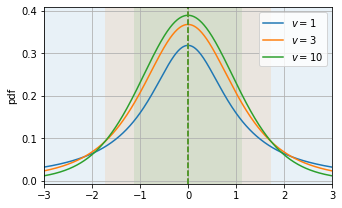
\includegraphics[width=0.32\textwidth]{pdf_t} &
            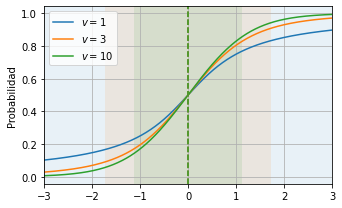
\includegraphics[width=0.32\textwidth]{cdf_t} \\
        \end{tabular}
    \end{center}
    \begin{block}{Propiedades}
        \begin{itemize}
            \item $\expecteddist{X \sim \tdist{\nu}}{X} = \mu_{X} = 0$.
            \item $\variancedist{X \sim \tdist{\nu}}{X} = \sigma^{2}_{X} = \begin{cases} + \infty \text{ si } \nu \leq 2 , \\ \frac{\nu}{\nu - 2} \text{ si } \nu > 2 \end{cases}$.
        \end{itemize}
    \end{block}
\end{frame}

\begin{frame}
    \frametitle{Intervalos de confianza}
    \begin{block}{Si no conocemos varianza $\sigma^{2}$ y queremos estimar $\mu$}
        \begin{itemize}
            \item Supongamos que $X^{\parens{i}}$ tiene distribución normal $\normal{\mu}{\sigma^{2}}$.
            \item Calculamos media y varianza muestrales $\bar{X}_{n}$ y $S^{2}_{n}$.
            \item Sabemos que $T = \frac{\sqrt{n} \parens{\bar{X}_{n} - \mu}}{\sqrt{S^{2}_{n}}}$ sigue distribución $\tdist{n - 1}$.
            \item Buscamos intervalo centrado para $T$: $\prob{-t_{\frac{\alpha}{2}} \leq T < t_{\frac{\alpha}{2}}} = 1 - \alpha$.
            \item Resolvemos para $\mu$:
                \begin{multline*}
                    \prob{- t_{\frac{\alpha}{2}} \leq \sqrt{n} \frac{\bar{X}_{n} - \mu}{\sqrt{S^{2}_{n}}} < t_{\frac{\alpha}{2}}}
                    = 1 - \alpha
                    \\
                    \Rightarrow
                    \bar{X}_{n} - \frac{\sqrt{S^{2}_{n}}}{\sqrt{n}} t_{\frac{\alpha}{2}} < \mu \leq \bar{X}_{n} + \frac{\sqrt{S^{2}_{n}}}{\sqrt{n}} t_{\frac{\alpha}{2}}
                    .
                \end{multline*}
        \end{itemize}
    \end{block}
%    \begin{center}
%        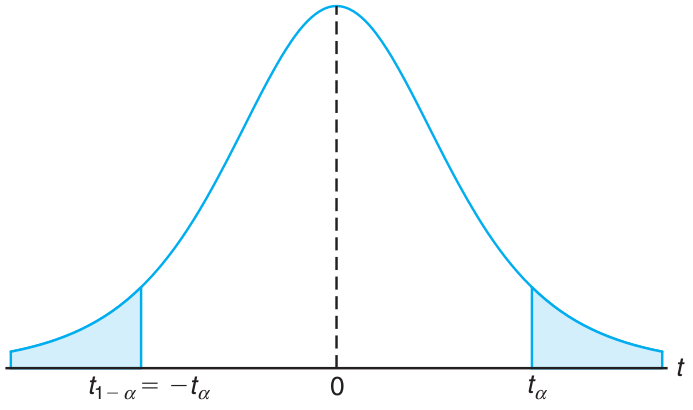
\includegraphics[height=0.15\textheight]{intervalo_t}
%    \end{center}

\begin{tikzpicture}[remember picture, overlay]
\node[yshift=1.4cm, xshift=-2cm] at (current page.south) 
{
    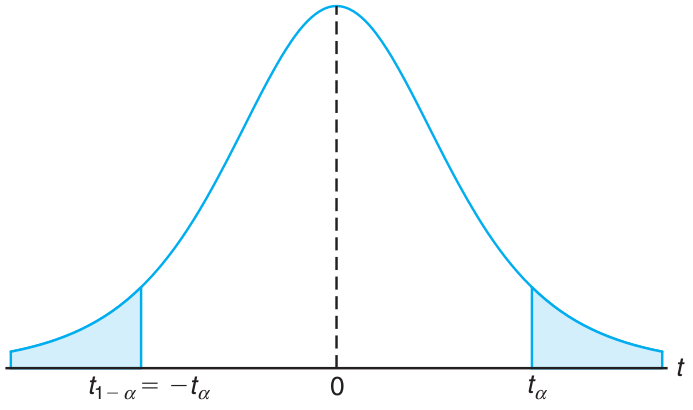
\includegraphics[width=0.4\textheight]{intervalo_t}
};
\end{tikzpicture}    

\end{frame}

\begin{frame}
    \frametitle{Intervalos de confianza}
    \begin{block}{Si conocemos $\mu$ y queremos estimar $\sigma^{2}$}
        \begin{itemize}
            \item Supongamos que $X^{\parens{i}}$ tiene distribución normal $\normal{\mu}{\sigma^{2}}$.
            \item Sabemos que $V =  \frac{\parens{n - 1} S^{2}_{n}}{\sigma^{2}}$ tiene distribución ji al cuadrado con $n - 1$ grados de libertad, $V \sim \chidist{n - 1}$.
            \item Buscamos intervalo centrado para $V$: $\prob{v_{\frac{\alpha}{2}} \leq V < v_{1 - \frac{\alpha}{2}}} = 1 - \alpha$.
            \item Resolvemos para $\sigma^{2}$:
                \begin{multline*}
                    \prob{v_{\frac{\alpha}{2}} \leq \frac{\parens{n - 1} S^{2}_{n}}{\sigma^{2}} < v_{1 - \frac{\alpha}{2}}}
                    = 1 - \alpha
                    \\
                    \Rightarrow
                    \frac{\parens{n - 1} S^{2}_{n}}{v_{\frac{1 - \alpha}{2}}} < \sigma^{2} \leq \frac{\parens{n - 1} S^{2}_{n}}{v_{\frac{\alpha}{2}}}
                    .
                \end{multline*}
        \end{itemize}
    \end{block}
%    \begin{center}
%        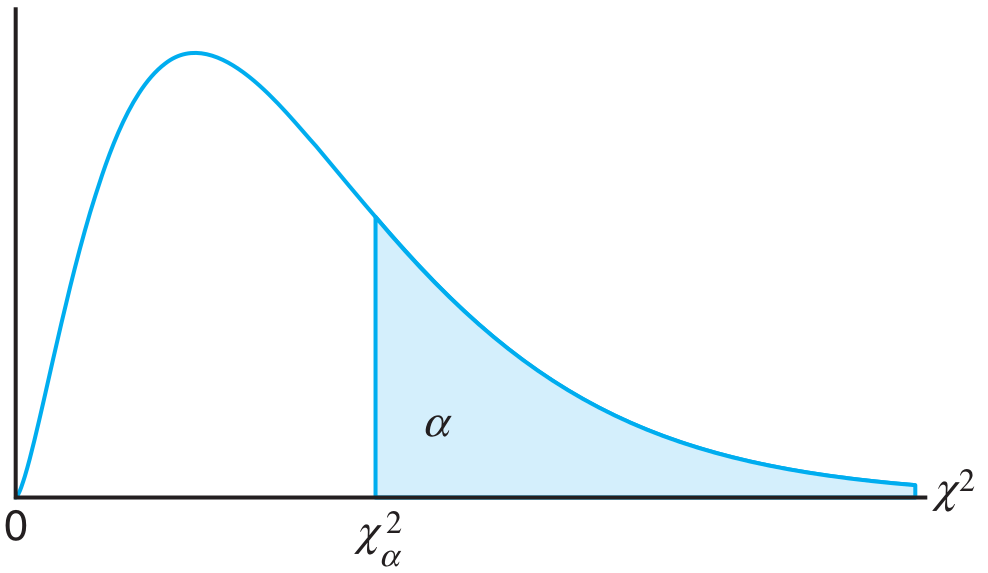
\includegraphics[height=0.2\textheight]{intervalo_chi}
%    \end{center}

\begin{tikzpicture}[remember picture, overlay]
\node[yshift=1.5cm, xshift=-2cm] at (current page.south) 
{
    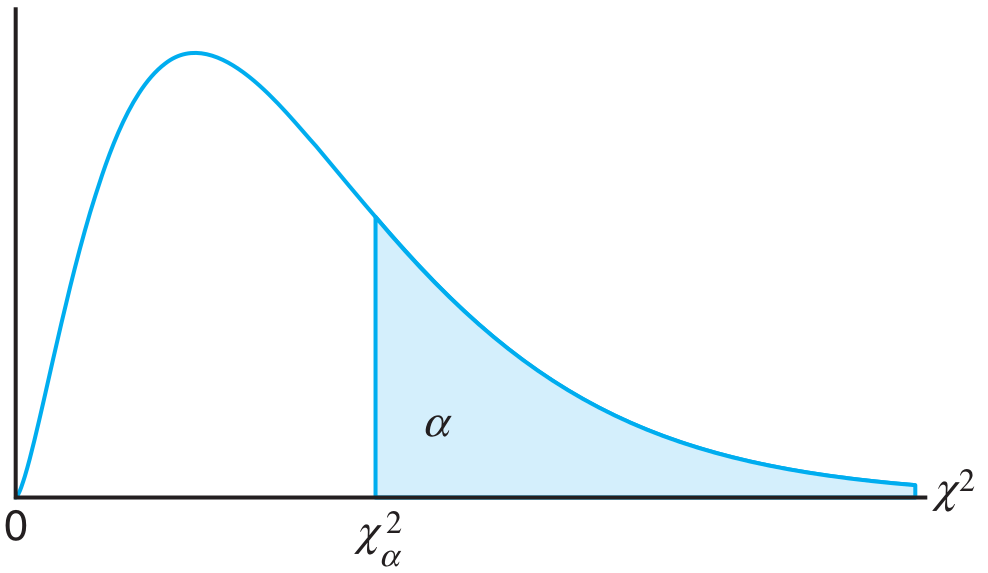
\includegraphics[width=0.5\textheight]{intervalo_chi}
};
\end{tikzpicture}    

\end{frame}

\begin{frame}
    \frametitle{Distribución ji al cuadrado $v$ grados de libertad $\chidist{v}$}
    \begin{block}{Definición}
        \begin{equation*}
            \pdf{x} = \frac{x^{\frac{v}{2} - 1} e^{- \frac{v}{2}}}{2^{\frac{v}{2}} \gammafunc{\frac{v}{2}}} .
        \end{equation*}
    \end{block}
    \begin{center}
        \begin{tabular}{cc}
            \emph{pdf} ($\pdf{x}$) & \emph{cdf} ($\FF{x}$) \\
            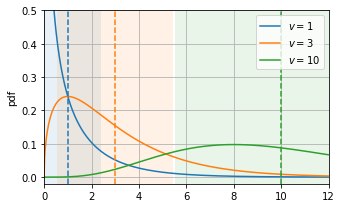
\includegraphics[width=0.32\textwidth]{pdf_chi2} &
            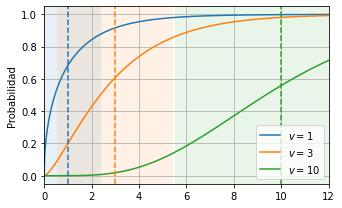
\includegraphics[width=0.32\textwidth]{cdf_chi2} \\
        \end{tabular}
    \end{center}
    \begin{block}{Propiedades}
        \begin{itemize}
            \item $\expecteddist{X \sim \chidist{v}}{X} = \mu_{X} = v$.
            \item $\variancedist{X \sim \chidist{v}}{X} = \sigma^{2}_{X} = 2 v$.
        \end{itemize}
    \end{block}
\end{frame}

\begin{frame}
    \frametitle{XKCD}
    \begin{center}
        
\includegraphics[width=\textwidth]{xkcd_t}
    \end{center}
\end{frame}

\begin{frame}
    \frametitle{Sesgo}
    \begin{block}{Estimador insesgado}
        \begin{itemize}
            \item Un estimador $\hat{\theta}$ es \emph{insesgado} si $\expected{\hat{\theta}} = \theta$ para cualquier valor de $\theta$.
            \item En caso contrario, el estimador es sesgado y $\expected{\hat{\theta}} - \theta$ se llama \emph{sesgo}.
        \end{itemize}
    \end{block}
    \begin{block}{Ejemplo: varianza muestral}
        \begin{itemize}
            \item Consideremos el siguiente estimador de la varianza:
                \begin{equation*}
                    \hat{\sigma}^{2}_{n} = \frac{1}{n} \sum_{i = 1}^{n} \parens{X^{\parens{i}} - \bar{X}_{n}}^{2} .
                \end{equation*}
            \item ¿Es sesgado?
        \end{itemize}
    \end{block}
\end{frame}

\begin{frame}
    \frametitle{Sesgo}
    \begin{block}{Ejemplo: varianza muestral}
        \begin{multline*}
            \expected{\hat{\sigma}^{2}_{n}} = \frac{1}{n} \sum_{i = 1}^{n} \expected{\parens{X^{\parens{i}} - \bar{X}_{n}}^{2}}
            = \frac{1}{n} \sum_{i = 1}^{n} \expected{X^{\parens{i} 2} + \bar{X}_{n}^{2} - 2 X^{\parens{i}} \bar{X}_{n}}
            \\
            = \frac{1}{n} \sum_{i = 1}^{n} \parens{\expected{X^{\parens{i} 2}} + \expected{\bar{X}_{n}^{2}} - 2 \expected{X^{\parens{i}} \bar{X}_{n}}}
            \\
            = \frac{1}{n} \sum_{i = 1}^{n} \parens{\expected{X^{\parens{i} 2}} + \expected{\frac{1}{n^{2}} \sum_{j = 1}^{n} \sum_{k = 1}^{n} X^{\parens{j}} X^{\parens{k}}} - 2 \expected{\frac{1}{n} X^{\parens{i}} \sum_{j = 1}^{n} X^{\parens{j}}}}
            \\
            %= \frac{1}{n} \sum_{i = 1}^{n} \parens{\sigma^{2} + \mu^{2} + \frac{1}{n^{2}} \parens{\parens{n^{2} - n} \mu^{2} + n \parens{\sigma^{2} + \mu^{2}}} - \frac{2}{n} \parens{\parens{n - 1} \mu^{2} + \sigma^{2} + \mu^{2}}}
        \end{multline*}
    \end{block}
\end{frame}

\begin{frame}
    \frametitle{Sesgo}
    \begin{block}{Ejemplo: varianza muestral}
        \begin{multline*}
                       %= \frac{1}{n} \sum_{i = 1}^{n} \parens{\sigma^{2} + \mu^{2} + \frac{1}{n^{2}} \parens{\parens{n^{2} - n} \mu^{2} + n \parens{\sigma^{2} + \mu^{2}}} - \frac{2}{n} \parens{\parens{n - 1} \mu^{2} + \sigma^{2} + \mu^{2}}}
            = \sum_{i = 1}^{n} \parens{\frac{\sigma^{2} + \mu^{2}}{n} + \frac{\parens{n^{2} - n} \mu^{2} + n \parens{\sigma^{2} + \mu^{2}}}{n^{3}} - \frac{2 \parens{\parens{n - 1} \mu^{2} + \sigma^{2} + \mu^{2}}}{n^{2}}}
            \\
            = \frac{1}{n^{2}} \parens{n^{2} \sigma^{2} + n^{2} \mu^{2} + n^{2} \mu^{2} + n \sigma^{2} - 2 n^{2} \mu^{2} - 2 n \sigma^{2}}
            \\
            = \frac{\parens{n^{2} - n}}{n^{2}} \sigma^{2} = \frac{n - 1}{n} \sigma^{2} .
        \end{multline*}
    \end{block}
\end{frame}

\begin{frame}
    \frametitle{Sesgo}
    \begin{block}{Ejemplo: varianza muestral}
        \begin{itemize}
            \item ¡El estimador $\hat{\sigma}^{2}_{n}$ es sesgado!
            \item $\expected{\hat{\sigma}^{2}_{n}} = \frac{n - 1}{n} \sigma^{2}$.
        \end{itemize}
    \end{block}
    \begin{block}{Corrección: varianza muestral con $n - 1$}
        \begin{itemize}
            \item Consideremos el siguiente estimador de la varianza:
                \begin{equation*}
                    S^{2}_{n} = \frac{1}{n - 1} \sum_{i = 1}^{n} \parens{X^{\parens{i}} - \bar{X}_{n}}^{2}
                    = \frac{n}{n - 1} \hat{\sigma}^{2}_{n} .
                \end{equation*}
            \item Ahora tenemos que:
                \begin{equation*}
                    \expected{S^{2}_{n}} = \frac{1}{n - 1} \expected{\hat{\sigma}^{2}_{n}}
                    = \frac{n}{n - 1} \frac{n - 1}{n} \sigma^{2}
                    = \sigma^{2} .
                \end{equation*}
        \end{itemize}
    \end{block}
\end{frame}

\begin{frame}
    \frametitle{Otros estimadores}
    \begin{block}{¿Cómo podemos obtener estimadores?}
        \begin{itemize}
            \item Minimizar una función de error.
            \item Máxima verosimilitud.
            \item Máximo a posteriori.
        \end{itemize}
    \end{block}
\end{frame}

\begin{frame}
    \frametitle{Estimador insesgado de mínima varianza (\emph{MVUE})}
    \begin{block}{Definición}
        \begin{itemize}
            \item Estimador insesgado de $\theta$:
                \begin{equation*}
                    \expected{\hat{\theta}} = \theta .
                \end{equation*}
            \item Menor varianza:
                \begin{equation*}
                    \hat{\theta} = \underset{e \text{ estimador insesgado}}{\arg \min} \expected{\parens{e - \theta}^{2}} .
                \end{equation*}
        \end{itemize}
    \end{block}
    \begin{center}
        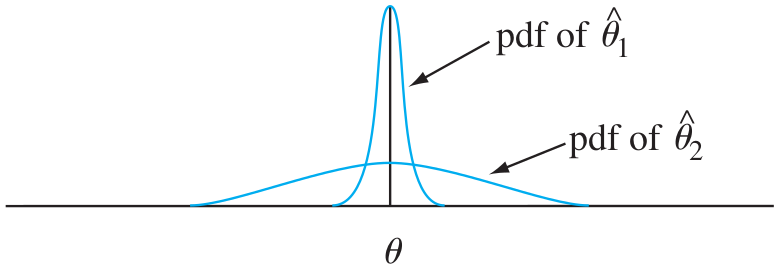
\includegraphics[height=0.26\textheight]{mvue}
    \end{center}
    \begin{block}{Nota}
        \begin{itemize}
            \item Si es que existe, es único. - No siempre existe.
        \end{itemize}
    \end{block}
\end{frame}

\begin{frame}
    \frametitle{Minimizar una función de error}
    \begin{block}{Error cuadático medio}
        \begin{itemize}
            \item Definición:
                \begin{equation*}
                    \text{MSE} \parens{\hat{\theta}} = \expected{\parens{\hat{\theta} - \theta}^{2}} .
                \end{equation*}
            \item Al igual que antes, se minimiza MSE:
                \begin{equation*}
                    \hat{\theta} = \underset{e \text{ estimador}}{\arg \min} \text{MSE} \parens{\hat{\theta}} = \underset{e \text{ estimador}}{\arg \min} \expected{\parens{e - \theta}^{2}} .
                \end{equation*}
        \end{itemize}
    \end{block}
    \begin{block}{Descomposición}
        \begin{multline*}
            \text{MSE} \parens{\hat{\theta}} = \expected{\parens{\hat{\theta} - \expected{\hat{\theta}} + \expected{\hat{\theta}} - \theta}^{2}}
            \\
            %= \expected{\parens{\hat{\theta} - \expected{\hat{\theta}}}^{2}} + \parens{\expected{\hat{\theta}} - \theta}^{2}
            %\\
            = \underbrace{\expected{\parens{\hat{\theta} - \expected{\hat{\theta}}}^{2}}}_{\text{varianza}} + \underbrace{\parens{\expected{\hat{\theta}} - \theta}^{2}}_{\text{sesgo}^{2}}
        \end{multline*}
    \end{block}
\end{frame}

\begin{frame}
    \frametitle{Minimizar una función de error}
    \begin{block}{Ejemplo}
        \begin{itemize}
            \item Sea $\hat{\theta}_{\text{MVUE}}$ el estimador insesgado de mínima varianza.
            \item Sea $\hat{\theta}_{\alpha} = \parens{1 + \alpha} \hat{\theta}_{\text{MVUE}}$ otro estimador.
            \item Notar que $\expected{\hat{\theta}_{\alpha}} = \parens{1 + \alpha} \theta$. Si $\alpha \neq 0$, es sesgado.
        \end{itemize}
    \end{block}
    \begin{block}{Se tiene que}
        \begin{equation*}
            \text{MSE} \parens{\hat{\theta}_{\alpha}} = \parens{1 + \alpha}^{2} \text{MSE} \parens{\hat{\theta}_{\text{MVUE}}} + \alpha^{2} \theta^{2} .
        \end{equation*}
    \end{block}
    \begin{block}{El error es menor si}
        \begin{equation*}
            - \frac{2 \text{MSE} \parens{\hat{\theta}_{\text{MVUE}}}}{\text{MSE} \parens{\hat{\theta}_{\text{MVUE}}} + \theta^{2}} < \alpha < 0 .
        \end{equation*}
    \end{block}
\end{frame}

\begin{frame}
    \frametitle{Consistencia}
    \begin{block}{Definición}
        \begin{itemize}
            \item Un estimador $\hat{\theta}_{n}$ es consistente si converge a $\theta$ cuando $n \to \infty$.
        \end{itemize}
    \end{block}
    \begin{block}{¿Por qué?}
        \begin{itemize}
            \item Todo estimador cuyo sesgo y varianza convergen a 0 si $n \to \infty$, es consistente.
            \item Un estimador insesgado lo es para todo $n$.
            \item Aquí nos interesa que sea bueno cuando $n$ es grande.
            \item La media muestral $\bar{X}_{n}$ es consistente.
        \end{itemize}
    \end{block}
\end{frame}

\begin{frame}
    \frametitle{Recordar -- estimadores}
    \begin{block}{Funciones de la muestra aleatoria}
        \begin{itemize}
            \item $\hat{\theta}_{n} = g \parens{X^{\parens{1}} , X^{\parens{2}} , \ldots , X^{\parens{n}}}$.
            \item Son variables aleatorias: tienen una distribución de probabilidad.
        \end{itemize}
    \end{block}
    \begin{center}
        \includegraphics[height=0.35\textheight]{sampling_distribution}
    \end{center}
    \begin{block}{En realidad no conocemos $\theta$}
        \begin{itemize}
            \item Bayes:
        \end{itemize}
        \begin{equation*}
            \pdf{\theta \mid \Xvec_{n}} = \frac{\pdf{\Xvec_{n} \mid \theta} \pdf{\theta}}{\pdf{\Xvec_{n}}} .
            %= \frac{\pdf{\Xvec_{n} \mid \theta} \pdf{\theta}}{\int_{- \infty}^{+ \infty} \pdf{\Xvec_{n} \mid \theta '} \pdf{\theta '} d \theta '} .
            %= \frac{\pdf{\Xvec_{n} \mid \theta} \pdf{\theta}}{\expecteddist{\theta ' \sim \pdf{\theta '}}{\pdf{\Xvec_{n} \mid \theta '}}} .
        \end{equation*}
    \end{block}
\end{frame}

\begin{frame}
    \frametitle{Enfoque bayesiano}
    \begin{block}{En realidad no conocemos $\theta$}
        \begin{equation*}
            \pdf{\theta \mid \Xvec_{n}} = \frac{\pdf{\Xvec_{n} \mid \theta} \pdf{\theta}}{\pdf{\Xvec_{n}}} .
            % = \frac{\pdf{\Xvec_{n} \mid \theta} \pdf{\theta}}{\int_{- \infty}^{+ \infty} \pdf{\Xvec_{n} \mid \theta '} \pdf{\theta '} d \theta '} .
        \end{equation*}
    \end{block}
    \begin{center}
        \includegraphics[height=0.5\textheight]{sampling_distribution}
    \end{center}
\end{frame}

\begin{frame}
    \frametitle{Ejemplo: modelo de distribución normal}
    \begin{block}{Datos}
        \begin{itemize}
            \item Logaritmo de cantidad de horas jugadas en promedio de $3000$ juegos de plataforma Steam.
        \end{itemize}
    \end{block}
    \begin{center}
        \includegraphics[height=0.4\textheight]{post_datos}
    \end{center}
    \begin{block}{Modelo}
        \begin{itemize}
            \item Supongamos un modelo como $\normal{\mu}{\sigma^{2}}$.
            \item Queremos estimar $\mu$ y $\sigma^{2}$.
        \end{itemize}
    \end{block}
\end{frame}

\iffalse
\begin{frame}
    \frametitle{Ejemplo: modelo de distribución normal}
    \begin{block}{Modelo}
        \begin{itemize}
            \item Supongamos un modelo como $\normal{\mu}{\sigma^{2}}$.
            \item Queremos estimar $\mu$ y $\sigma^{2}$.
        \end{itemize}
    \end{block}
    \begin{center}
        \includegraphics[height=0.4\textheight]{post_datos}
    \end{center}
    \begin{block}{Distribución conjunta de $\mu$ y $\sigma^{2}$}
        \begin{equation*}
            \pdf{\mu , \sigma^{2} \mid \Xvec_{n}} = \frac{\pdf{\Xvec_{n} \mid \mu , \sigma^{2}} \pdf{\mu , \sigma^{2}}}{\pdf{\Xvec_{n}}} .
            % \pdf{\mu \mid \Xvec_{n}} = \frac{\pdf{\Xvec_{n} \mid \mu} \pdf{\mu}}{\pdf{\Xvec_{n}}} \text{ y }
            % \pdf{\sigma^{2} \mid \Xvec_{n}} = \frac{\pdf{\Xvec_{n} \mid \sigma^{2}} \pdf{\sigma^{2}}}{\pdf{\Xvec_{n}}} .
        \end{equation*}
    \end{block}
\end{frame}
\fi

\begin{frame}
    \frametitle{Ejemplo: modelo de distribución normal $\normal{\mu}{\sigma^{2}}$}
    \begin{block}{Distribución conjunta de $\mu$ y $\sigma^{2}$}
        \begin{equation*}
            \pdf{\mu , \sigma^{2} \mid \Xvec_{n}} = \frac{\overbrace{\pdf{\Xvec_{n} \mid \mu , \sigma^{2}}}^{\text{verosimilitud}} \overbrace{\pdf{\mu , \sigma^{2}}}^{\text{a priori}}}{\underbrace{\pdf{\Xvec_{n}}}_{\text{evidencia}}} .
            % \pdf{\mu \mid \Xvec_{n}} = \frac{\pdf{\Xvec_{n} \mid \mu} \pdf{\mu}}{\pdf{\Xvec_{n}}} \text{ y }
            % \pdf{\sigma^{2} \mid \Xvec_{n}} = \frac{\pdf{\Xvec_{n} \mid \sigma^{2}} \pdf{\sigma^{2}}}{\pdf{\Xvec_{n}}} .
        \end{equation*}
    \end{block}
    \begin{block}{Componentes}
        \begin{itemize}
            \item Verosimilitud:
                %\begin{equation*}
                %    \pdf{\Xvec_{n} \mid \mu} = \int_{0}^{+ \infty} \pdf{\Xvec_{n} \mid \mu , \sigma^{2}} \pdf{\sigma^{2}} d \sigma^{2} .
                %\end{equation*}
                %\begin{equation*}
                %    \pdf{\Xvec_{n} \mid \sigma^{2}} = \int_{- \infty}^{+ \infty} \pdf{\Xvec_{n} \mid \mu , \sigma^{2}} \pdf{\mu} d \mu .
                %\end{equation*}
                \begin{equation*}
                    \pdf{\Xvec_{n} \mid \mu , \sigma^{2}}
                        = \prod_{i = 1}^{n} \pdf{x^{\parens{i}} \mid \mu , \sigma^{2}}
                        = \prod_{i = 1}^{n} \frac{1}{\sqrt{2 \pi \sigma^{2}}} e^{- \frac{\parens{x^{\parens{i}} - \mu}^{2}}{2 \sigma^{2}}} .
                \end{equation*}
           
           
        \end{itemize}
    \end{block}
\end{frame}
\begin{frame}
    \frametitle{Ejemplo: modelo de distribución normal $\normal{\mu}{\sigma^{2}}$}
    
    \begin{block}{Componentes}
        \begin{itemize}
         
            \item A priori: veremos dos casos:
                \begin{enumerate}
                    \item $\mu \sim \normal{0}{1}$ y $\sigma^{2} \sim \gammadist{1.5}{0.01}$.
                    \item $\mu \sim \uniform{-4}{4}$ y $\sigma^{2} \sim \uniform{0.1}{2}$.
                \end{enumerate}
            \item Evidencia: cte. de normalización para $\iint \pdf{\mu , \sigma^{2} \mid \Xvec_{n}} d \mu d \sigma^{2} = 1$.
        \end{itemize}
    \end{block}
\end{frame}


\begin{frame}
    \frametitle{Ejemplo: modelo de distribución normal $\normal{\mu}{\sigma^{2}}$}
    \begin{center}
        \begin{tabular}{cccc}
            \multirow{2}{*}{\rotatebox[origin=c]{90}{Caso 1}} &
            \multirow{2}{*}[14mm]{\includegraphics[height=0.4\textheight]{post_prior_d}} &
            \includegraphics[height=0.2\textheight]{post_priorex1} &
            \includegraphics[height=0.2\textheight]{post_priorex2} \\
            & &
            \includegraphics[height=0.2\textheight]{post_priorex3} &
            \includegraphics[height=0.2\textheight]{post_priorex4} \\
            \hline
            \hline
            \multirow{2}{*}{\rotatebox[origin=c]{90}{Caso 2}} &
            \multirow{2}{*}[14mm]{\includegraphics[height=0.4\textheight]{post_priorunif_d}} &
            \includegraphics[height=0.2\textheight]{post_priorunifex1} &
            \includegraphics[height=0.2\textheight]{post_priorunifex2} \\
            & &
            \includegraphics[height=0.2\textheight]{post_priorunifex3} &
            \includegraphics[height=0.2\textheight]{post_priorunifex4} \\
        \end{tabular}
    \end{center}
\end{frame}

\begin{frame}
    \frametitle{Ejemplo: modelo de distribución normal $\normal{\mu}{\sigma^{2}}$}
    \begin{center}
        \begin{tabular}{cm{4cm}m{6cm}}
            \rotatebox[origin=c]{90}{Caso 1} &
            \includegraphics[height=0.4\textheight]{post_prior_d} &
            \includegraphics[height=0.4\textheight]{post_prior_h} \\
            \hline
            \hline
            \rotatebox[origin=c]{90}{Caso 2} &
            \includegraphics[height=0.4\textheight]{post_priorunif_d} &
            \includegraphics[height=0.4\textheight]{post_priorunif_h} \\
        \end{tabular}
    \end{center}
\end{frame}

\iffalse
\begin{frame}
    \frametitle{Ejemplo: modelo de distribución normal $\normal{\mu}{\sigma^{2}}$}
    \begin{center}
        \begin{tabular}{cc}
            Caso 1 & Caso 2 \\
            \includegraphics[height=0.45\textheight]{post_prior_d} &
            \includegraphics[height=0.45\textheight]{post_priorunif_d} \\
            \includegraphics[height=0.34\textheight]{post_prior_h} &
            \includegraphics[height=0.34\textheight]{post_priorunif_h} \\
        \end{tabular}
    \end{center}
\end{frame}
\fi

\begin{frame}
    \frametitle{Ejemplo: modelo de distribución normal -- caso 1}
    \begin{center}
        \begin{tabular}{cccc}
            a priori & 1 dato & 2 datos & 3 datos \\
            \includegraphics[height=0.21\textheight]{post_prior_d} &
            \includegraphics[height=0.21\textheight]{post_1_d} &
            \includegraphics[height=0.21\textheight]{post_2_d} &
            \includegraphics[height=0.21\textheight]{post_3_d} \\
            \includegraphics[height=0.15\textheight]{post_prior_h} &
            \includegraphics[height=0.15\textheight]{post_1_h} &
            \includegraphics[height=0.15\textheight]{post_2_h} &
            \includegraphics[height=0.15\textheight]{post_3_h} \\
            5 datos & 10 datos & 100 datos & 3000 datos \\
            \includegraphics[height=0.21\textheight]{post_5_d} &
            \includegraphics[height=0.21\textheight]{post_10_d} &
            \includegraphics[height=0.21\textheight]{post_100_d} &
            \includegraphics[height=0.21\textheight]{post_3000_d} \\
            \includegraphics[height=0.15\textheight]{post_5_h} &
            \includegraphics[height=0.15\textheight]{post_10_h} &
            \includegraphics[height=0.15\textheight]{post_100_h} &
            \includegraphics[height=0.15\textheight]{post_3000_h} \\
        \end{tabular}
    \end{center}
\end{frame}

\begin{frame}
    \frametitle{Ejemplo: modelo de distribución normal -- caso 2}
    \begin{center}
        \begin{tabular}{cccc}
            a priori & 1 dato & 2 datos & 3 datos \\
            \includegraphics[height=0.21\textheight]{post_priorunif_d} &
            \includegraphics[height=0.21\textheight]{post_unif1_d} &
            \includegraphics[height=0.21\textheight]{post_unif2_d} &
            \includegraphics[height=0.21\textheight]{post_unif3_d} \\
            \includegraphics[height=0.15\textheight]{post_priorunif_h} &
            \includegraphics[height=0.15\textheight]{post_unif1_h} &
            \includegraphics[height=0.15\textheight]{post_unif2_h} &
            \includegraphics[height=0.15\textheight]{post_unif3_h} \\
            5 datos & 10 datos & 100 datos & 3000 datos \\
            \includegraphics[height=0.21\textheight]{post_unif5_d} &
            \includegraphics[height=0.21\textheight]{post_unif10_d} &
            \includegraphics[height=0.21\textheight]{post_unif100_d} &
            \includegraphics[height=0.21\textheight]{post_unif3000_d} \\
            \includegraphics[height=0.15\textheight]{post_unif5_h} &
            \includegraphics[height=0.15\textheight]{post_unif10_h} &
            \includegraphics[height=0.15\textheight]{post_unif100_h} &
            \includegraphics[height=0.15\textheight]{post_unif3000_h} \\
        \end{tabular}
    \end{center}
\end{frame}

\begin{frame}
    \frametitle{Enfoque bayesiano}
    \begin{block}{Distribución de $\theta$}
        \begin{equation*}
            \pdf{\theta \mid \Xvec_{n}} = \frac{\pdf{\Xvec_{n} \mid \theta} \pdf{\theta}}{\pdf{\Xvec_{n}}} .
            % = \frac{\pdf{\Xvec_{n} \mid \theta} \pdf{\theta}}{\int_{- \infty}^{+ \infty} \pdf{\Xvec_{n} \mid \theta '} \pdf{\theta '} d \theta '} .
        \end{equation*}
    \end{block}
    \begin{center}
        \includegraphics[height=0.3\textheight]{sampling_distribution}
        \includegraphics[height=0.3\textheight]{post_3000_d}
    \end{center}
    \begin{block}{Una posibilidad: buscar el máximo de $\pdf{\theta \mid \Xvec_{n}}$}
        \begin{multline*}
            \hat{\theta}_{n} = \arg \max_{\theta} \pdf{\theta \mid \Xvec_{n}} = \arg \max_{\theta} \frac{\pdf{\Xvec_{n} \mid \theta} \pdf{\theta}}{\pdf{\Xvec_{n}}}
            \\
            = \arg \max_{\theta} \pdf{\Xvec_{n} \mid \theta} \pdf{\theta} .
        \end{multline*}
    \end{block}
\end{frame}

\begin{frame}
    \frametitle{Máxima verosimilitud (\emph{Maximum likelihood estimate MLE})}
    \begin{center}
        \includegraphics[height=0.35\textheight]{sampling_distribution}
        \includegraphics[height=0.35\textheight]{post_3000_d}
    \end{center}
    \begin{block}{Máximo de $\pdf{\theta \mid \Xvec_{n}}$}
        \begin{itemize}
            \item En este enfoque, se ignora la distribución a priori.
            \item En caso de que $\theta$ es acotado, sería equivalente a una distribución uniforme a priori.
        \end{itemize}
        \begin{equation*}
            \hat{\theta}_{n}
            = \arg \max_{\theta} \pdf{\Xvec_{n} \mid \theta} .
        \end{equation*}
    \end{block}
\end{frame}

\begin{frame}
    \frametitle{Máxima verosimilitud (\emph{Maximum likelihood estimate MLE})}
    \begin{block}{Máximo de $\pdf{\theta \mid \Xvec_{n}}$}
        \begin{equation*}
            \hat{\theta}_{n}
            = \arg \max_{\theta} \pdf{\Xvec_{n} \mid \theta} .
        \end{equation*}
    \end{block}
    \begin{exampleblock}{Ejemplo: modelo de distribución normal $\normal{\mu}{\sigma^{2}}$}
        \begin{itemize}
            \item Verosimilitud:
                \begin{equation*}
                    \pdf{\Xvec_{n} \mid \mu , \sigma^{2}}
                    = \prod_{i = 1}^{n} \pdf{x^{\parens{i}} \mid \mu , \sigma^{2}}
                    = \prod_{i = 1}^{n} \frac{1}{\sqrt{2 \pi \sigma^{2}}} e^{- \frac{\parens{x^{\parens{i}} - \mu}^{2}}{2 \sigma^{2}}} .
                \end{equation*}
            \item Maximizamos logaritmo con respecto a $\mu$, derivando e igualando a $0$:
                \begin{equation*}
                    \frac{d \sparens{\ln \parens{\pdf{\Xvec_{n} \mid \mu , \sigma^{2}}}}}{d \mu}
                    = \sum_{i = 1}^{n} \frac{1}{\sigma^{2}} \parens{x^{\parens{i}} - \mu}
                    = 0
                    \Rightarrow \hat{\mu}_{n} = \frac{1}{n} \sum_{i = 1}^{n} x^{\parens{i}} .
                \end{equation*}
        \end{itemize}
    \end{exampleblock}
\end{frame}

\begin{frame}
    \frametitle{Máxima verosimilitud (\emph{Maximum likelihood estimate MLE})}
    \begin{block}{Máximo de $\pdf{\theta \mid \Xvec_{n}}$}
        \begin{equation*}
            \hat{\theta}_{n}
            = \arg \max_{\theta} \pdf{\Xvec_{n} \mid \theta} .
        \end{equation*}
    \end{block}
    \begin{exampleblock}{Ejemplo: modelo de distribución normal $\normal{\mu}{\sigma^{2}}$}
        \begin{equation*}
            \pdf{\Xvec_{n} \mid \mu , \sigma^{2}}
            = \prod_{i = 1}^{n} \pdf{x^{\parens{i}} \mid \mu , \sigma^{2}}
            = \prod_{i = 1}^{n} \frac{1}{\sqrt{2 \pi \sigma^{2}}} e^{- \frac{\parens{x^{\parens{i}} - \mu}^{2}}{2 \sigma^{2}}} .
        \end{equation*}
        \begin{itemize}
            \item Maximizamos logaritmo con respecto a $\sigma^{2}$, derivando e igualando a $0$:
                \begin{multline*}
                    \frac{d \sparens{\ln \parens{\pdf{\Xvec_{n} \mid \mu , \sigma^{2}}}}}{d \sigma^{2}}
                    = \sum_{i = 1}^{n} \frac{d}{d \sigma^{2}} \sparens{- \frac{1}{2} \parens{\ln \parens{\sigma^{2}} + \frac{\parens{x^{\parens{i}} - \mu}^{2}}{\sigma^{2}}}}
                    \\
                    = \sum_{i = 1}^{n} - \frac{1}{2} \parens{\frac{1}{\sigma^{2}} - \frac{\parens{x^{\parens{i}} - \mu}^{2}}{\parens{\sigma^{2}}^{2}}}
                    = 0
                    \Rightarrow \hat{\sigma}^{2}_{n} = \frac{1}{n} \sum_{i = 1}^{n} \parens{x^{\parens{i}} - \mu}^{2} .
                \end{multline*}
        \end{itemize}
    \end{exampleblock}
\end{frame}

\begin{frame}
    \frametitle{Máxima verosimilitud (\emph{Maximum likelihood estimate MLE})}
    \begin{block}{Máximo de $\pdf{\theta \mid \Xvec_{n}}$}
        \begin{equation*}
            \hat{\theta}_{n}
            = \arg \max_{\theta} \pdf{\Xvec_{n} \mid \theta} .
        \end{equation*}
    \end{block}
    \begin{exampleblock}{Ejemplo: modelo de distribución normal $\normal{\mu}{\sigma^{2}}$}
        \begin{itemize}
            \item Estimadores de máxima verosimilitud (\emph{MLE}):
                \begin{equation*}
                    \hat{\mu}_{n} = \frac{1}{n} \sum_{i = 1}^{n} x^{\parens{i}} \text{ y }
                    \hat{\sigma}^{2}_{n} = \frac{1}{n} \sum_{i = 1}^{n} \parens{x^{\parens{i}} - \mu}^{2} .
                \end{equation*}
        \end{itemize}
    \end{exampleblock}
    \begin{center}
        \includegraphics[height=0.35\textheight]{mle}
    \end{center}
\end{frame}

\begin{frame}
    \frametitle{Máxima verosimilitud (\emph{Maximum likelihood estimate MLE})}
    \begin{block}{Máximo de $\pdf{\theta \mid \Xvec_{n}}$}
        \begin{itemize}
            \item En este enfoque, se ignora la distribución a priori.
            \item En caso de que $\theta$ es acotado, sería equivalente a una distribución uniforme a priori.
        \end{itemize}
        \begin{equation*}
            \hat{\theta}_{n}
            = \arg \max_{\theta} \pdf{\Xvec_{n} \mid \theta} .
        \end{equation*}
    \end{block}
    \begin{block}{Propiedades}
        \begin{itemize}
            \item Es asintóticamente insesgado: $\lim_{n \to \infty} \expected{\hat{\theta}_{n}} = \theta$.
            \item Es asintóticamente consistente: $\lim_{n \to \infty} \prob{\vparens{\hat{\theta}_{n} - \theta} > \epsilon} = 0$.
            \item Es \emph{eficiente} (su varianza es la menor posible para un estimador insesgado. Buscar teorema de Cramér-Rao).
            \item Si existe un estadístico suficiente para $\theta$, el estimador de máxima verosimilitud se puede expresar en base a ese estadístico.
        \end{itemize}
    \end{block}
\end{frame}

\begin{frame}
    \frametitle{Máxima verosimilitud (\emph{Maximum likelihood estimate MLE})}
    \begin{exampleblock}{Ejemplo: distribución de Poisson}
        \begin{itemize}
            \item Muestra $\bparens{x^{\parens{1}} , \ldots , x^{\parens{n}}}$ de tamaño $n$.
            \item Recordar: $\ff{x^{\parens{i}}} = e^{- \lambda} \frac{\lambda^{x^{\parens{i}}}}{x^{\parens{i}} !}$.
            \item ¿Estimador $\hat{\lambda}_{n}^{\text{MLE}}$ de $\lambda$?
        \end{itemize}
    \end{exampleblock}
    \begin{block}{Desarrollo}
        \begin{itemize}
            \item Verosimilitud:
                \begin{equation*}
                    \prob{\Xvec_{n} \mid \lambda} = \prod_{i = 1}^{n} e^{- \lambda} \frac{\lambda^{x^{\parens{i}}}}{x^{\parens{i}} !} = e^{- \lambda n} \frac{\lambda^{\sum_{i = 1}^{n} x^{\parens{i}}}}{\prod_{i = 1}^{n} x^{\parens{i}} !} .
                \end{equation*}
            \item Maximizamos derivando con respecto a $\lambda$ e igualando a $0$:
                \begin{equation*}
                    \parens{- n + \frac{1}{\lambda} \sum_{i = 1}^{n} x^{\parens{i}}} e^{- \lambda n + \ln{\parens{\lambda}} \sum_{i = 1}^{n} x^{\parens{i}}} = 0 \Rightarrow \hat{\lambda}_{n}^\text{MLE} = \frac{1}{n} \sum_{i = 1}^{n} x^{\parens{i}} .
                \end{equation*}
        \end{itemize}
    \end{block}
\end{frame}

\begin{frame}
    \frametitle{Máxima verosimilitud (\emph{Maximum likelihood estimate MLE})}
    \begin{exampleblock}{Ejemplo: distribución Gamma}
        \begin{itemize}
            \item Muestra $\bparens{x^{\parens{1}} , \ldots , x^{\parens{n}}}$ de tamaño $n$.
            \item Recordar: $\pdf{x^{\parens{i}}} = \frac{\beta^{\alpha}}{\gammafunc{\alpha}} {x^{\parens{i}}}^{\alpha - 1} e^{- \beta x^{\parens{i}}}$.
            \item ¿Estimador $\hat{\beta}_{n}^{\text{MLE}}$ de $\beta$, si $\alpha$ es conocido?
        \end{itemize}
    \end{exampleblock}
    \begin{block}{Desarrollo}
        \begin{itemize}
            \item Verosimilitud:
                \begin{equation*}
                    \pdf{\Xvec_{n} \mid \alpha, \beta} = \prod_{i = 1}^{n} \frac{\beta^{\alpha}}{\gammafunc{\alpha}} {x^{\parens{i}}}^{\alpha - 1} e^{- \beta x^{\parens{i}}} = \frac{\beta^{\alpha n} e^{- \beta \sum_{i = 1}^{n} x^{\parens{i}}}}{\gammafunc{\alpha}^{n}} \prod_{i = 1}^{n} {x^{\parens{i}}}^{\alpha - 1} .
                \end{equation*}
            \item Maximizamos derivando con respecto a $\beta$ e igualando a $0$:
                \begin{equation*}
                    \parens{\frac{\alpha n}{\beta} - \sum_{i = 1}^{n} x^{\parens{i}}} e^{- \beta \sum_{i = 1}^{n} x^{\parens{i}} + \ln{\parens{\beta}} \alpha n} = 0 \Rightarrow \hat{\beta}_{n}^\text{MLE} = \frac{\alpha n}{\sum_{i = 1}^{n} x^{\parens{i}}} .
                \end{equation*}
        \end{itemize}
    \end{block}
\end{frame}

\begin{frame}
    \frametitle{Enfoque bayesiano}
    \begin{block}{Distribución de $\theta$}
        \begin{equation*}
            \pdf{\theta \mid \Xvec_{n}} = \frac{\pdf{\Xvec_{n} \mid \theta} \pdf{\theta}}{\pdf{\Xvec_{n}}} .
            % = \frac{\pdf{\Xvec_{n} \mid \theta} \pdf{\theta}}{\int_{- \infty}^{+ \infty} \pdf{\Xvec_{n} \mid \theta '} \pdf{\theta '} d \theta '} .
        \end{equation*}
    \end{block}
    \begin{center}
        \includegraphics[height=0.3\textheight]{sampling_distribution}
        \includegraphics[height=0.3\textheight]{post_3000_d}
    \end{center}
    \begin{block}{Una posibilidad: buscar el máximo de $\pdf{\theta \mid \Xvec_{n}}$}
        \begin{multline*}
            \hat{\theta}_{n} = \arg \max_{\theta} \pdf{\theta \mid \Xvec_{n}} = \arg \max_{\theta} \frac{\pdf{\Xvec_{n} \mid \theta} \pdf{\theta}}{\pdf{\Xvec_{n}}}
            \\
            = \arg \max_{\theta} \pdf{\Xvec_{n} \mid \theta} \pdf{\theta} .
        \end{multline*}
    \end{block}
\end{frame}

\begin{frame}
    \frametitle{Máximo a posteriori (\emph{Maximum a posteriori MAP})}
    \begin{center}
        \includegraphics[height=0.35\textheight]{sampling_distribution}
        \includegraphics[height=0.35\textheight]{post_3000_d}
    \end{center}
    \begin{block}{Máximo de $\pdf{\theta \mid \Xvec_{n}}$}
        \begin{itemize}
            \item En este enfoque, se debe definir un a priori.
            \item Como vimos, es más importante cuando $n$ es pequeño.
        \end{itemize}
        \begin{equation*}
            \hat{\theta}_{n}
            = \arg \max_{\theta} \pdf{\Xvec_{n} \mid \theta} \pdf{\theta} .
        \end{equation*}
    \end{block}
\end{frame}

\begin{frame}
    \frametitle{Máximo a posteriori (\emph{Maximum a posteriori MAP})}
    \begin{block}{Máximo de $\pdf{\theta \mid \Xvec_{n}}$}
        \begin{equation*}
            \hat{\theta}_{n}
            = \arg \max_{\theta} \pdf{\Xvec_{n} \mid \theta} \pdf{\theta} .
        \end{equation*}
    \end{block}
    \begin{exampleblock}{Ejemplo: modelo de distribución normal $\normal{\mu}{\sigma^{2}}$ y prior $\normal{0}{1}$}
        \begin{equation*}
            \pdf{\Xvec_{n} \mid \mu , \sigma^{2}}
            \pdf{\mu , \sigma^{2}}
            = \pdf{\sigma^{2}} \frac{1}{\sqrt{2 \pi}} e^{- \frac{\mu^{2}}{2}} \prod_{i = 1}^{n} \frac{1}{\sqrt{2 \pi \sigma^{2}}} e^{- \frac{\parens{x^{\parens{i}} - \mu}^{2}}{2 \sigma^{2}}} .
        \end{equation*}
        \begin{itemize}
            \item Supongamos $\sigma^{2}$ conocido, y estimemos $\mu$:
                \begin{equation*}
                    \pdf{\Xvec_{n} \mid \mu}
                    \pdf{\mu}
                    = \frac{1}{\sqrt{2 \pi}} e^{- \frac{\mu^{2}}{2}} \prod_{i = 1}^{n} \frac{1}{\sqrt{2 \pi \sigma^{2}}} e^{- \frac{\parens{x^{\parens{i}} - \mu}^{2}}{2 \sigma^{2}}} .
                \end{equation*}
        \end{itemize}
    \end{exampleblock}
\end{frame}

\begin{frame}
    \frametitle{Máximo a posteriori (\emph{Maximum a posteriori MAP})}
    \begin{block}{Máximo de $\pdf{\theta \mid \Xvec_{n}}$}
        \begin{equation*}
            \hat{\theta}_{n}
            = \arg \max_{\theta} \pdf{\Xvec_{n} \mid \theta} \pdf{\theta} .
        \end{equation*}
    \end{block}
    \begin{exampleblock}{Ejemplo: modelo de distribución normal $\normal{\mu}{\sigma^{2}}$ y prior $\normal{0}{1}$}
        \begin{equation*}
            \pdf{\Xvec_{n} \mid \mu}
            \pdf{\mu}
            = \frac{1}{\sqrt{2 \pi}} e^{- \frac{\mu^{2}}{2}} \prod_{i = 1}^{n} \frac{1}{\sqrt{2 \pi \sigma^{2}}} e^{- \frac{\parens{x^{\parens{i}} - \mu}^{2}}{2 \sigma^{2}}} .
        \end{equation*}
        \begin{itemize}
            %\item Supongamos $\sigma^{2}$ conocido, y estimemos $\mu$:
            \item Maximizamos logaritmo con respecto a $\mu$, derivando e igualando a $0$:
                \begin{multline*}
                    \frac{d \sparens{\ln \parens{\pdf{\Xvec_{n} \mid \mu , \sigma^{2}} \pdf{\mu , \sigma^{2}}}}}{d \mu}
                    = - \mu + \sum_{i = 1}^{n} \frac{1}{\sigma^{2}} \parens{x^{\parens{i}} - \mu}
                    = 0
                    \\
                    \Rightarrow \hat{\mu}_{n} = \frac{1}{n + \sigma^{2}} \sum_{i = 1}^{n} x^{\parens{i}} .
                \end{multline*}
        \end{itemize}
    \end{exampleblock}
\end{frame}

\begin{frame}
    \frametitle{Máximo a posteriori (\emph{Maximum a posteriori MAP})}
    \begin{block}{Máximo de $\pdf{\theta \mid \Xvec_{n}}$}
        \begin{equation*}
            \hat{\theta}_{n}
            = \arg \max_{\theta} \pdf{\Xvec_{n} \mid \theta} \pdf{\theta} .
        \end{equation*}
    \end{block}
    \begin{exampleblock}{Ejemplo: modelo de distribución normal $\normal{\mu}{\sigma^{2}}$ y prior $\normal{0}{1}$}
        \begin{itemize}
            \item Suponiendo:
                \begin{itemize}
                    \item $\sigma^{2}$ conocido.
                    \item A priori $\mu \sim \normal{0}{1}$.
                \end{itemize}
            \item Entonces el estimador de máximo a posteriori (\emph{MAP}) de $\mu$ es:
                \begin{equation*}
                    \hat{\mu}_{n} = \frac{1}{n + \sigma^{2}} \sum_{i = 1}^{n} x^{\parens{i}} .
                \end{equation*}
        \end{itemize}
    \end{exampleblock}
\end{frame}

\begin{frame}
    \frametitle{Ejemplo: Modelo de lenguaje GPT-3}
    \begin{center}
        \scriptsize
        \begin{tabular}{lrcrcrrc}
        Model Name & $n_{\text{params}}$ & $n_{\text{layers}}$ & $d_{\text{model}}$ & $n_{\text{heads}}$ & $d_{\text{head}}$  & Batch Size & Learning Rate \\
        \hline
GPT-3 Small & $125$ M & $12$ & $768$ & $12$ & $64$ & $0.5$ M & $6.0 \times 10^{-4}$ \\
GPT-3 Med. & $350$ M & $24$ & $1024$ & $16$ & $64$ & $0.5$ M & $3.0 \times 10^{-4}$ \\
GPT-3 Large & $760$ M & $24$ & $1536$ & $16$ & $96$ & $0.5$ M & $2.5 \times 10^{-4}$ \\
GPT-3 XL & $1.3$ B & $24$ & $2048$ & $24$ & $128$ & $1$ M & $2.0 \times 10^{-4}$ \\
GPT-3 2.7B   & $2.7$ B & $32$ & $2560$ & $32$ & $80$ & $1$ M & $1.6 \times 10^{-4}$ \\
GPT-3 6.7B   & $6.7$ B & $32$ & $4096$ & $32$ & $128$ & $2$ M & $1.2 \times 10^{-4}$ \\
GPT-3 13B  & $13.0$ B & $40$ & $5140$ & $40$ & $128$ & $2$ M & $1.0 \times 10^{-4}$ \\
GPT-3 175B & $175.0$ B & $96$ & $12288$ & $96$ & $128$ & $3.2$ M & $0.6 \times 10^{-4}$ \\
o ``GPT-3'' & & & & & & &
        \end{tabular}
        \includegraphics[height=0.47\textheight]{gpt3_training_flops}
    \end{center}
\end{frame}

\begin{frame}
    \frametitle{Aplicación: mezcla de Gaussianas}
    \begin{exampleblock}{Ejemplo}
        \begin{itemize}
            \item Se desea modelar una varibale aleatoria con un modelo de \emph{mezcla de dos Gaussianas}:
                \begin{equation*}
                    \pdf{x \mid \mu_{1} , \mu_{2} , \sigma^{2}} = \sum_{k = 1}^{2} \pi_{k} \frac{1}{\sqrt{2 \pi \sigma^{2}}} e^{- \frac{\parens{x - \mu_{k}}^{2}}{2 \sigma^{2}}} .
                \end{equation*}
            \item $k = 1 , 2$ indica la etiqueta de la Guassiana.
            \item Ambas tienen la misma varianza $\sigma^{2}$, pero distintas medias $\mu_{1}$ y $\mu_{2}$.
            \item Se supone una probabilidad a priori para cada clase $\pi_{1} = \frac{1}{2}$ y $\pi_{2} = \frac{1}{2}$.
            \item Se tiene una muestra iid de $N$ datos, donde cada uno proviene de una Gaussiana.
            %\item Llamamos $\mathbf{\theta} = \bparens{\sigma^{2} , \mu_{1} , \mu_{2}}$.
        \end{itemize}
    \end{exampleblock}
\end{frame}

\begin{frame}
    \frametitle{Aplicación: mezcla de Gaussianas}
    \begin{exampleblock}{Modelo}
        \begin{equation*}
            \pdf{x \mid \mu_{1} , \mu_{2} , \sigma^{2}} = \sum_{k = 1}^{2} \pi_{k} \frac{1}{\sqrt{2 \pi \sigma^{2}}} e^{- \frac{\parens{x - \mu_{k}}^{2}}{2 \sigma^{2}}} .
        \end{equation*}
    \end{exampleblock}
    \begin{center}
        \begin{tikzpicture}[
            declare function={normal(\x,\m,\s) = 1 / (\s * sqrt(2 * pi)) * exp(-(\x - \m)^2 / (2 * \s^2));
            mixture(\m,\s,\n,\t,\p) = \p * normal(x, \m, \s) + (1 - \p) * normal(x, \n, \t);}]
            \begin{axis}[
                clip=false,
                axis lines=left,
%                scaled ticks=false,
                domain=0:12,
                samples=100,
                xlabel=$X$,
                ylabel=$\pdf{x}$,
                %extra y ticks={0},
                %extra tick style={grid=major},
                legend entries={Component $1$,Component $2$,Mixture},
                ymin=-0.01,%, ymax=0.4
                height=0.65\textheight
                %xtick=\empty, ytick=\empty]
                ]
                \addplot[thick, blue] {normal(x, 3, 1)};
                \addplot[thick, orange] {normal(x, 7, 1.8)};
                \addplot[thick, dashed, black] {mixture(3, 1, 7, 1.8, 0.4)};
                \node[pin=270:$\mu^{\parens{1}}$] at (axis cs:3, {normal(3, 3, 1)}) {};
                \node (s1) at (axis cs:3, 0.04) {$\sigma^{\parens{1}}$};
                \node[pin=270:$\mu^{\parens{2}}$] at (axis cs:7, {normal(7, 7, 1.8)}) {};
                \node (s2) at (axis cs:7, 0.05) {$\sigma^{\parens{2}}$};
                \draw[->] (s1) -- (axis cs:0.95, 0.04);
                \draw[->] (s1) -- (axis cs:5.05, 0.04);
                \draw[->] (s2) -- (axis cs:4, 0.05);
                \draw[->] (s2) -- (axis cs:10, 0.05);
            \end{axis}
        \end{tikzpicture}
    \end{center}
\end{frame}

\begin{frame}
    \frametitle{Aplicación: mezcla de Gaussianas}
    \begin{exampleblock}{Modelo}
        \begin{equation*}
            \pdf{x \mid \mu_{1} , \mu_{2} , \sigma^{2}} = \sum_{k = 1}^{2} \frac{1}{2} \frac{1}{\sqrt{2 \pi \sigma^{2}}} e^{- \frac{\parens{x - \mu_{k}}^{2}}{2 \sigma^{2}}} .
        \end{equation*}
    \end{exampleblock}
    \begin{center}
        \includegraphics[height=0.5\textheight]{figure155}
    \end{center}
\end{frame}

\begin{frame}
    \frametitle{Aplicación: mezcla de Gaussianas}
    \begin{exampleblock}{Modelo}
        \begin{equation*}
            \pdf{x \mid \mu_{1} , \mu_{2} , \sigma^{2}} = \sum_{k = 1}^{2} \frac{1}{2} \frac{1}{\sqrt{2 \pi \sigma^{2}}} e^{- \frac{\parens{x - \mu_{k}}^{2}}{2 \sigma^{2}}} .
        \end{equation*}
    \end{exampleblock}
    \begin{block}{Posterior de clases}
        \begin{itemize}
            \item Sea $k_{i}$ la clase asociada al dato $i$.
        \end{itemize}
        \begin{multline*}
            p^{\parens{i}}_{1} = \pdf{k_{i} = 1 \mid x^{\parens{i}} , \mu_{1} , \mu_{2} , \sigma^{2}}
            \\
            = \frac{\pdf{x^{\parens{i}} \mid k_{i} = 1 , \mu_{1} , \mu_{2} , \sigma^{2}} \pdf{k_{i} = 1}}{\pdf{x^{\parens{i}} \mid \mu_{1} , \mu_{2}, \sigma^{2}}}
            \\
            = \frac{\frac{1}{\sqrt{2 \pi \sigma^{2}}} e^{- \frac{\parens{x - \mu_{1}}^{2}}{2 \sigma^{2}}} \frac{1}{2}}{\frac{1}{\sqrt{2 \pi \sigma^{2}}} e^{- \frac{\parens{x - \mu_{1}}^{2}}{2 \sigma^{2}}} \frac{1}{2} + \frac{1}{\sqrt{2 \pi \sigma^{2}}} e^{- \frac{\parens{x - \mu_{2}}^{2}}{2 \sigma^{2}}} \frac{1}{2}}
            = \frac{e^{- \frac{\parens{x - \mu_{1}}^{2}}{2 \sigma^{2}}}}{e^{- \frac{\parens{x - \mu_{1}}^{2}}{2 \sigma^{2}}} + e^{- \frac{\parens{x - \mu_{2}}^{2}}{2 \sigma^{2}}}}
        \end{multline*}
    \end{block}
\end{frame}

\begin{frame}
    \frametitle{Aplicación: mezcla de Gaussianas}
    \begin{exampleblock}{Modelo}
        \begin{equation*}
            \pdf{x \mid \mu_{1} , \mu_{2} , \sigma^{2}} = \sum_{k = 1}^{2} \frac{1}{2} \frac{1}{\sqrt{2 \pi \sigma^{2}}} e^{- \frac{\parens{x - \mu_{k}}^{2}}{2 \sigma^{2}}} .
        \end{equation*}
    \end{exampleblock}
    \begin{block}{Posterior de clases}
        \begin{equation*}
            p^{\parens{i}}_{1}% = \pdf{k_{i} = 1 \mid x^{\parens{i}} , \mathbf{\theta}}
            = \frac{e^{- \frac{\parens{x - \mu_{1}}^{2}}{2 \sigma^{2}}}}{e^{- \frac{\parens{x - \mu_{1}}^{2}}{2 \sigma^{2}}} + e^{- \frac{\parens{x - \mu_{2}}^{2}}{2 \sigma^{2}}}}
            = \frac{1}{1 + e^{\frac{2 x^{\parens{i}} \parens{\mu_{2} - \mu_{1}} - \parens{\mu_{2}^{2} - \mu_{1}^{2}}}{2 \sigma^{2}}}} ,
        \end{equation*}
        \begin{equation*}
            p^{\parens{i}}_{2}%\pdf{k_{i} = 2 \mid x , \mathbf{\theta}}
            = \frac{1}{1 + e^{\frac{- 2 x^{\parens{i}} \parens{\mu_{2} - \mu_{1}} + \parens{\mu_{2}^{2} - \mu_{1}^{2}}}{2 \sigma^{2}}}} .
        \end{equation*}
    \end{block}
\end{frame}

\begin{frame}
    \frametitle{Aplicación: mezcla de Gaussianas}
    \begin{exampleblock}{Modelo}
        \begin{equation*}
            \pdf{x \mid \mu_{1} , \mu_{2} , \sigma^{2}} = \sum_{k = 1}^{2} \frac{1}{2} \frac{1}{\sqrt{2 \pi \sigma^{2}}} e^{- \frac{\parens{x - \mu_{k}}^{2}}{2 \sigma^{2}}} .
        \end{equation*}
    \end{exampleblock}
    
\end{frame}

\begin{frame}
    \frametitle{Aplicación: mezcla de Gaussianas}
    
    \begin{block}{Si no conocemos $\mu_{1}$ y $\mu_{2}$}
        \begin{itemize}
            \item Los buscamos por MLE (máxima verosimilitud):
        \end{itemize}
        \begin{multline*}
            \frac{d}{d \mu_{k}} \ln \prod_{i = 1}^{n} \pdf{x^{\parens{i}} \mid \mu_{1} , \mu_{2} , \sigma^{2}} = \sum_{i = 1}^{n} \frac{d}{d \mu_{k}} \ln \sparens{\sum_{k' = 1}^{2} \frac{1}{2} \frac{1}{\sqrt{2 \pi \sigma^{2}}} e^{- \frac{\parens{x^{\parens{i}} - \mu_{k'}}^{2}}{2 \sigma^{2}}}}
            \\
            = \sum_{i = 1}^{n} \frac{\frac{1}{2} \parens{x^{\parens{i}} - \mu_{k}} e^{- \frac{\parens{x^{\parens{i}} - \mu_{k}}^{2}}{2 \sigma^{2}}}}{\sqrt{2 \pi \sigma^{2}} \sigma^{2} \sparens{\frac{1}{2 \sqrt{2 \pi \sigma^{2}}} e^{- \frac{\parens{x^{\parens{i}} - \mu_{1}}^{2}}{2 \sigma^{2}}} + \frac{1}{2 \sqrt{2 \pi \sigma^{2}}} e^{- \frac{\parens{x^{\parens{i}} - \mu_{2}}^{2}}{2 \sigma^{2}}}}}
            % \pdf{x^{\parens{i}} \mid \mu_{1} , \mu_{2}, \sigma^{2}}}
            \\
            = \sum_{i = 1}^{n} p^{\parens{i}}_{k} \frac{\parens{x^{\parens{i}} - \mu_{k}}}{\sigma^{2}}
            = 0
            .
        \end{multline*}
    \end{block}
\end{frame}

\begin{frame}
    \frametitle{Aplicación: mezcla de Gaussianas}
    \begin{exampleblock}{Modelo}
        \begin{equation*}
            \pdf{x \mid \mu_{1} , \mu_{2} , \sigma^{2}} = \sum_{k = 1}^{2} \frac{1}{2} \frac{1}{\sqrt{2 \pi \sigma^{2}}} e^{- \frac{\parens{x - \mu_{k}}^{2}}{2 \sigma^{2}}} .
        \end{equation*}
    \end{exampleblock}
    \begin{block}{Si no conocemos $\mu_{1}$ y $\mu_{2}$}
        \begin{itemize}
            \item Tenemos que $\hat{\mu}_{k} = \frac{\sum_{i = 1}^{n} p^{\parens{i}}_{k} x^{\parens{i}}}{\sum_{i = 1}^{n} p^{\parens{i}}_{k}}$, una media muestral ``con pesos''.
            \item Pero $p^{\parens{i}}_{k}$ depende de $\mu_{k}$.
            \item Se resuelve con algoritmo que actualiza $p^{\parens{i}}_{k}$ y $\hat{\mu}_{k}$ iterativamente.
        \end{itemize}
    \end{block}
    \begin{block}{Ejercicio}
        \begin{itemize}
            \item Verifique que la segunda derivada de la verosimilitud es negativa (es un máximo local).
        \end{itemize}
    \end{block}
\end{frame}

\begin{frame}
    \frametitle{Aplicación: mezcla de Gaussianas}
    \begin{exampleblock}{Modelo}
        \begin{equation*}
            \pdf{x \mid \mu_{1} , \mu_{2} , \sigma^{2}} = \sum_{k = 1}^{2} \frac{1}{2} \frac{1}{\sqrt{2 \pi \sigma^{2}}} e^{- \frac{\parens{x - \mu_{k}}^{2}}{2 \sigma^{2}}} .
        \end{equation*}
    \end{exampleblock}
    \begin{center}
        \includegraphics[width=\textwidth]{kmeans}
    \end{center}
\end{frame}

\begin{frame}
    \frametitle{Aplicación: mezcla de Gaussianas}
    \begin{exampleblock}{Modelo}
        \begin{equation*}
            \pdf{x \mid \mu_{1} , \mu_{2} , \sigma^{2}} = \sum_{k = 1}^{2} \frac{1}{2} \frac{1}{\sqrt{2 \pi \sigma^{2}}} e^{- \frac{\parens{x - \mu_{k}}^{2}}{2 \sigma^{2}}} .
        \end{equation*}
    \end{exampleblock}
    \begin{center}
        \includegraphics[width=\textwidth]{figure158}
    \end{center}
\end{frame}

\begin{frame}
    \frametitle{Aplicación: mezcla de Gaussianas}
    \begin{exampleblock}{Modelo}
        \begin{equation*}
            \pdf{x \mid \mu_{1} , \mu_{2} , \sigma^{2}} = \sum_{k = 1}^{2} \frac{1}{2} \frac{1}{\sqrt{2 \pi \sigma^{2}}} e^{- \frac{\parens{x - \mu_{k}}^{2}}{2 \sigma^{2}}} .
        \end{equation*}
    \end{exampleblock}
    \begin{center}
        \includegraphics[width=\textwidth]{figure159-1}
    \end{center}
\end{frame}

\begin{frame}
    \frametitle{Aplicación: mezcla de Gaussianas}
    \begin{exampleblock}{Modelo}
        \begin{equation*}
            \pdf{x \mid \mu_{1} , \mu_{2} , \sigma^{2}_{1} , \sigma^{2}_{2}} = \sum_{k = 1}^{2} \frac{1}{2} \frac{1}{\sqrt{2 \pi \sigma^{2}_{k}}} e^{- \frac{\parens{x - \mu_{k}}^{2}}{2 \sigma^{2}_{k}}} .
        \end{equation*}
    \end{exampleblock}
    \begin{center}
        \includegraphics[width=\textwidth]{kmeans}
    \end{center}
\end{frame}

\iffalse
\begin{frame}[allowframebreaks, noframenumbering]
\frametitle<presentation>{References}
\printbibliography
%\bibliographystyle{apalike}
\end{frame}
\fi

\end{document}